



We include a series of saliency maps  in the following 8 figures. Several interesting behavioral patterns can be observed. The figures are organized by model and by classification as follows: TN ---\autoref{fig:saliency_3id_contour} and \autoref{fig:saliency_nodia3id_contour}---, TP ---\autoref{fig:saliency_dia3id_TP} and \autoref{fig:tpndia}---, FN \autoref{fig:saliency_dia3id_FN} and \autoref{fig:fnndia}–––, and FP ---\autoref{fig:saliency_dia3id_FP} and \autoref{fig:fpndia}.

In  \autoref{fig:saliency_3id_contour} and \autoref{fig:saliency_nodia3id_contour} we include the transient's contours overplotted onto the saliency maps for the \diabased\ and \nodia\ model respectively to guide the reader's eye. 
% We note a few intriguing features and speculate on their meaning. In \autoref{fig:saliency_3id_contour}A, a dipole, the important pixels are located off-center, in correspondence to the dark portion of the dipole (althought we note that this classification is incorrect \fed{can you add a dipole with correct classification?}). 
Notice the offset of the \diabased\ model's focus in  \autoref{fig:saliency_3id_contour}A with respect to the transient: the model is principally inspecting the \diff\ and \temp\ at the location corresponding to the bright patch in the \diff.
In  \autoref{fig:saliency_3id_contour}C a correctly predicted ``bogus'', characterized by a very tight dipole probably arising from a poorly centered DIA, the saliency map inspect the \temp\ and even seem to reproduce traditional aperture photometry, with pixel values measured at the core of the transients, and in the sky surrounding the transients, but away from the tails of the bright pixels cluster. The behavior is principally different for the same transients when they are inspected, and also correctly predicted, by the \nodia\ model (\autoref{fig:saliency_nodia3id_contour}): the focus of the model is in all three cases away from the transients, and shifted to the surrounding: the model is learning the transients' context and extracting information to enable the comparison of \temp\ and \diff\ (essentially, to enable the image differencing). This behavior is generally seen throughout all examples in the following figures. In addition, for each figure we highlight potential reasons for failed predictions, and potential inaccuracies in the labeling that may lead to an artificial lowering of our measured accuracy.



\begin{figure*}
    \centering
    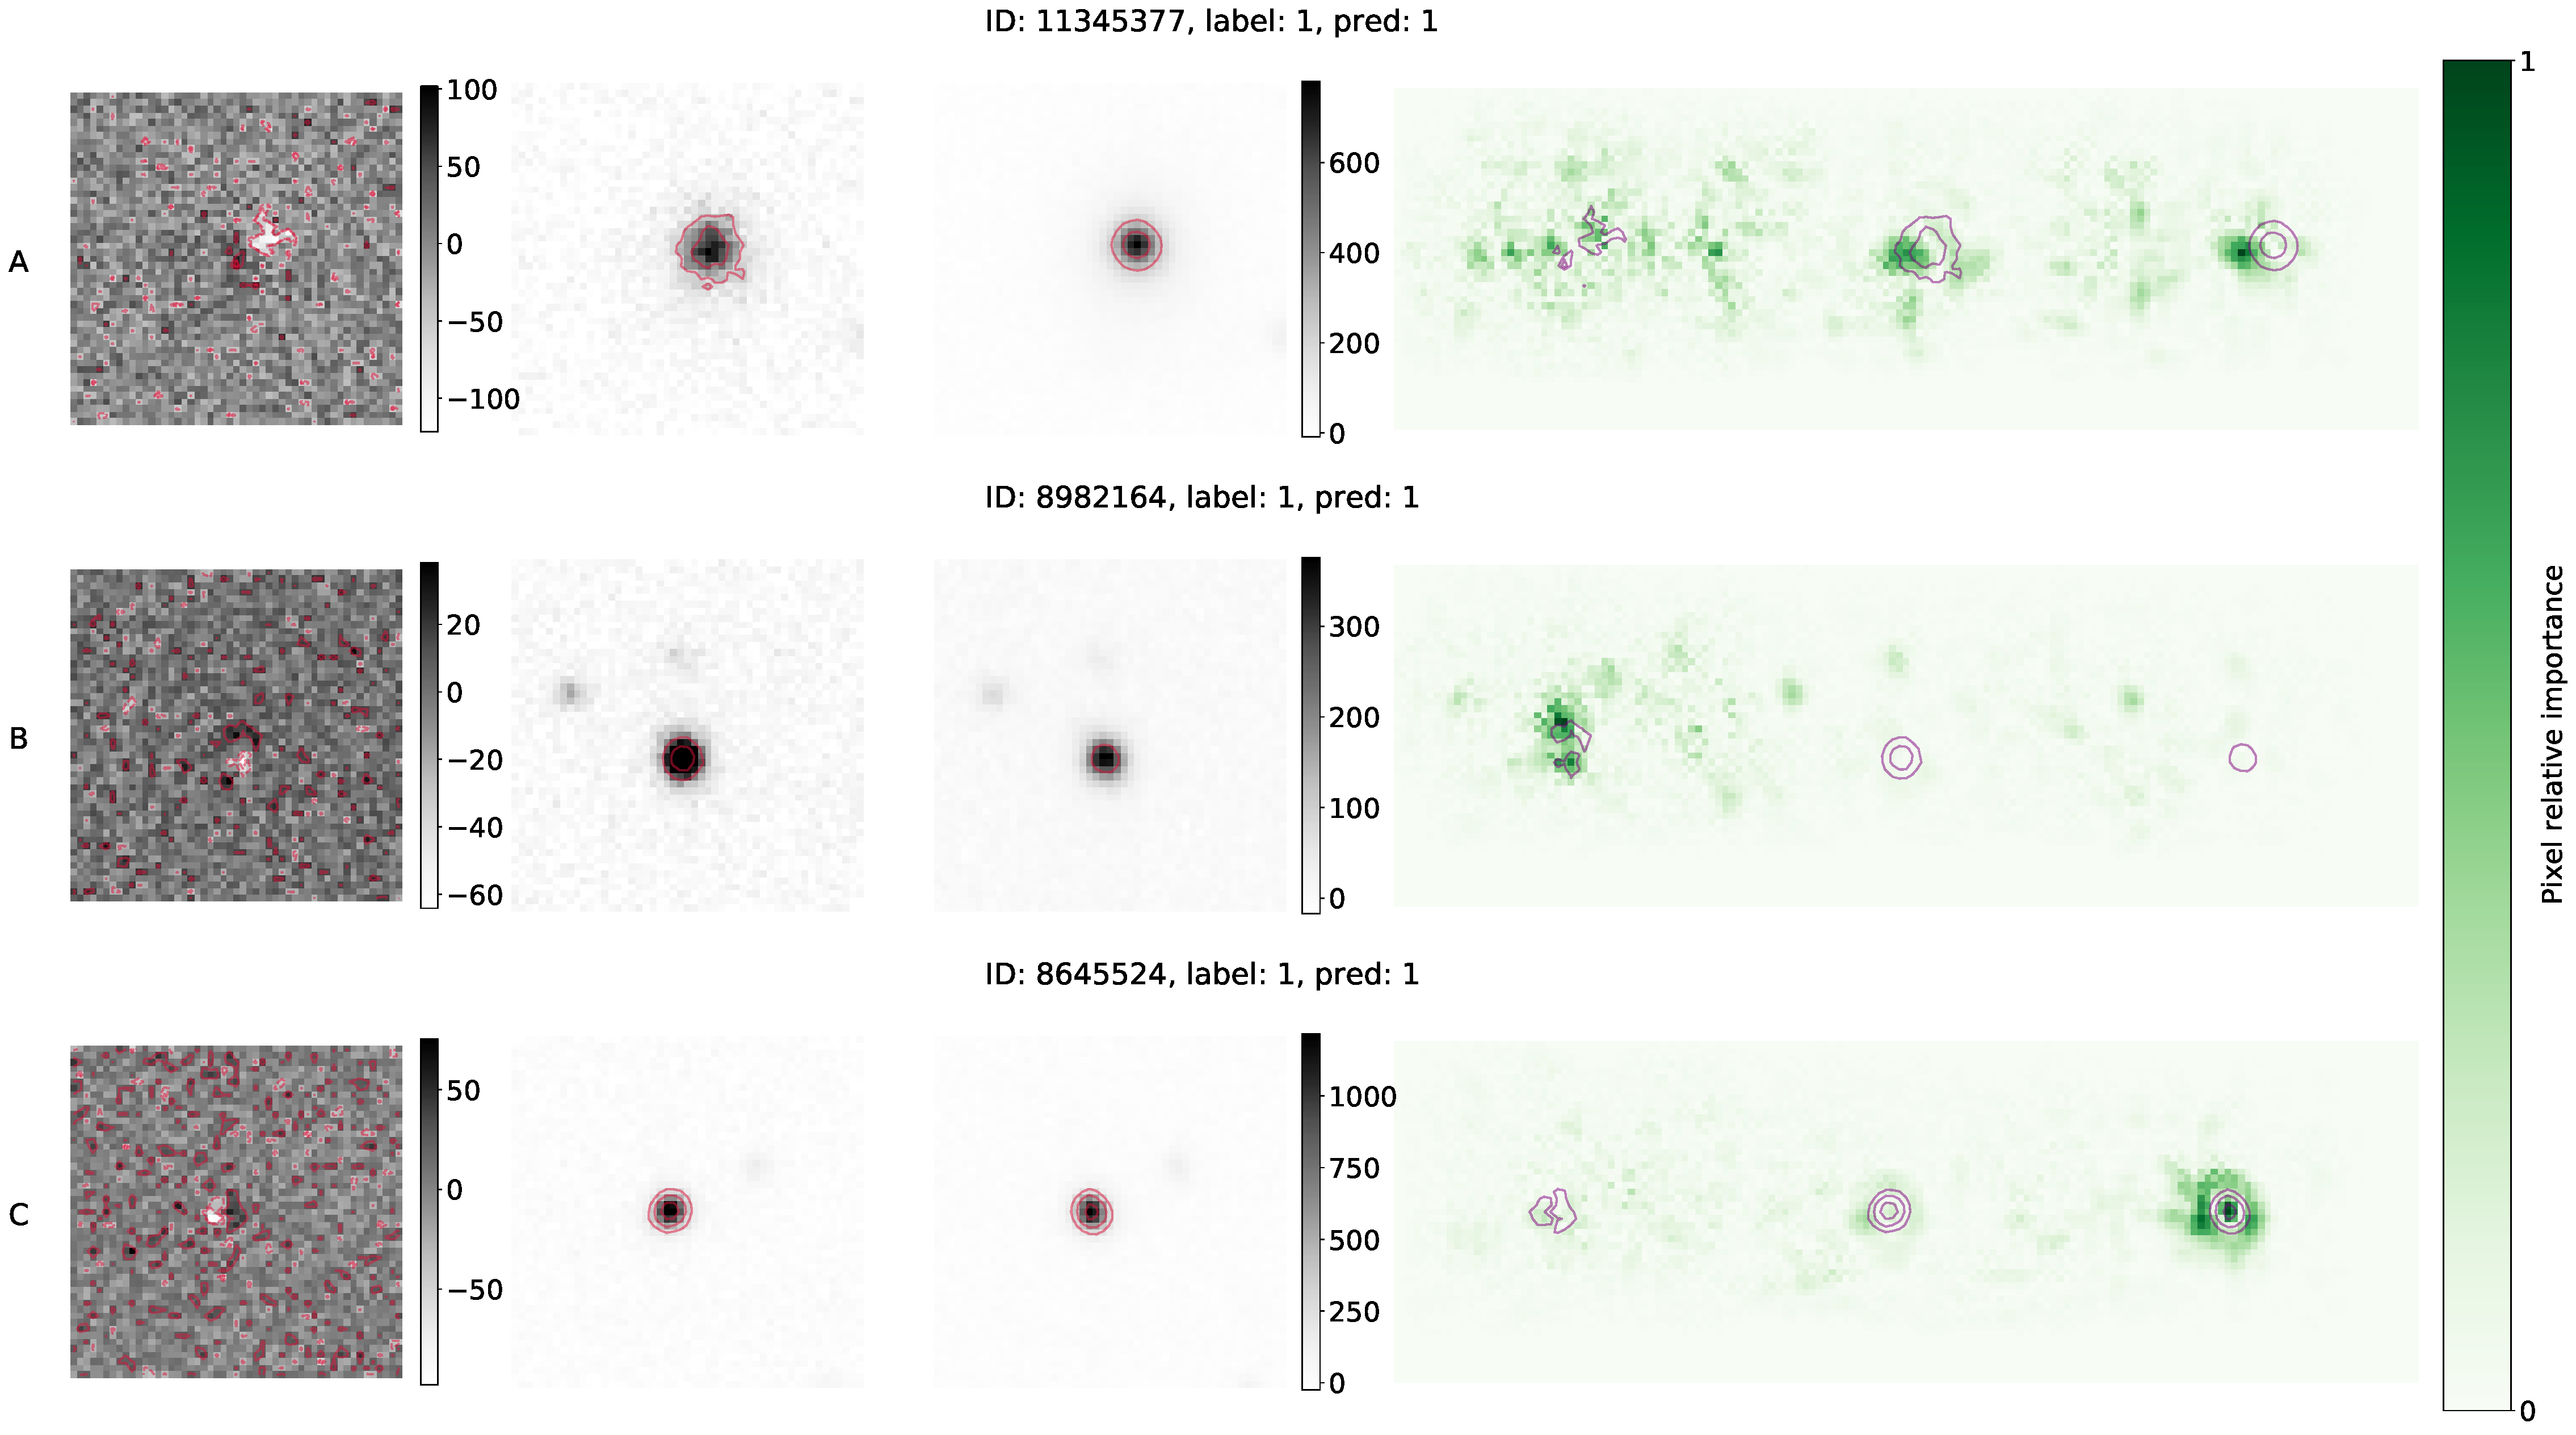
\includegraphics[width=0.85\linewidth]{
    figures/saliency_plot_3exam_contou_cheating.pdf}
    \caption{Transients (\diff-\search-\temp) and their respective saliency map for \diabased\ model True Negative predictions (correctly identified ``bogus'').  Contour plot of light intensity from the original images are overplotted, delineating the bright sources. In panel A: $I_\diff \sim 0.4$; B: $I_\diff\sim0.69$ and C $I_\temp\sim0.42$. In panel C, the saliency for the \temp\ portion of the image looks strikingly similar to the selection of pixels that is made in aperture photometry, with pixel values considered in the core of the source, ignored in a region immediately around the source, and again considered farther out to calculate the source's background. This figure is further discussed in \hyperref[sec:appendixc]{Appendix C}.}
    \label{fig:saliency_3id_contour}

    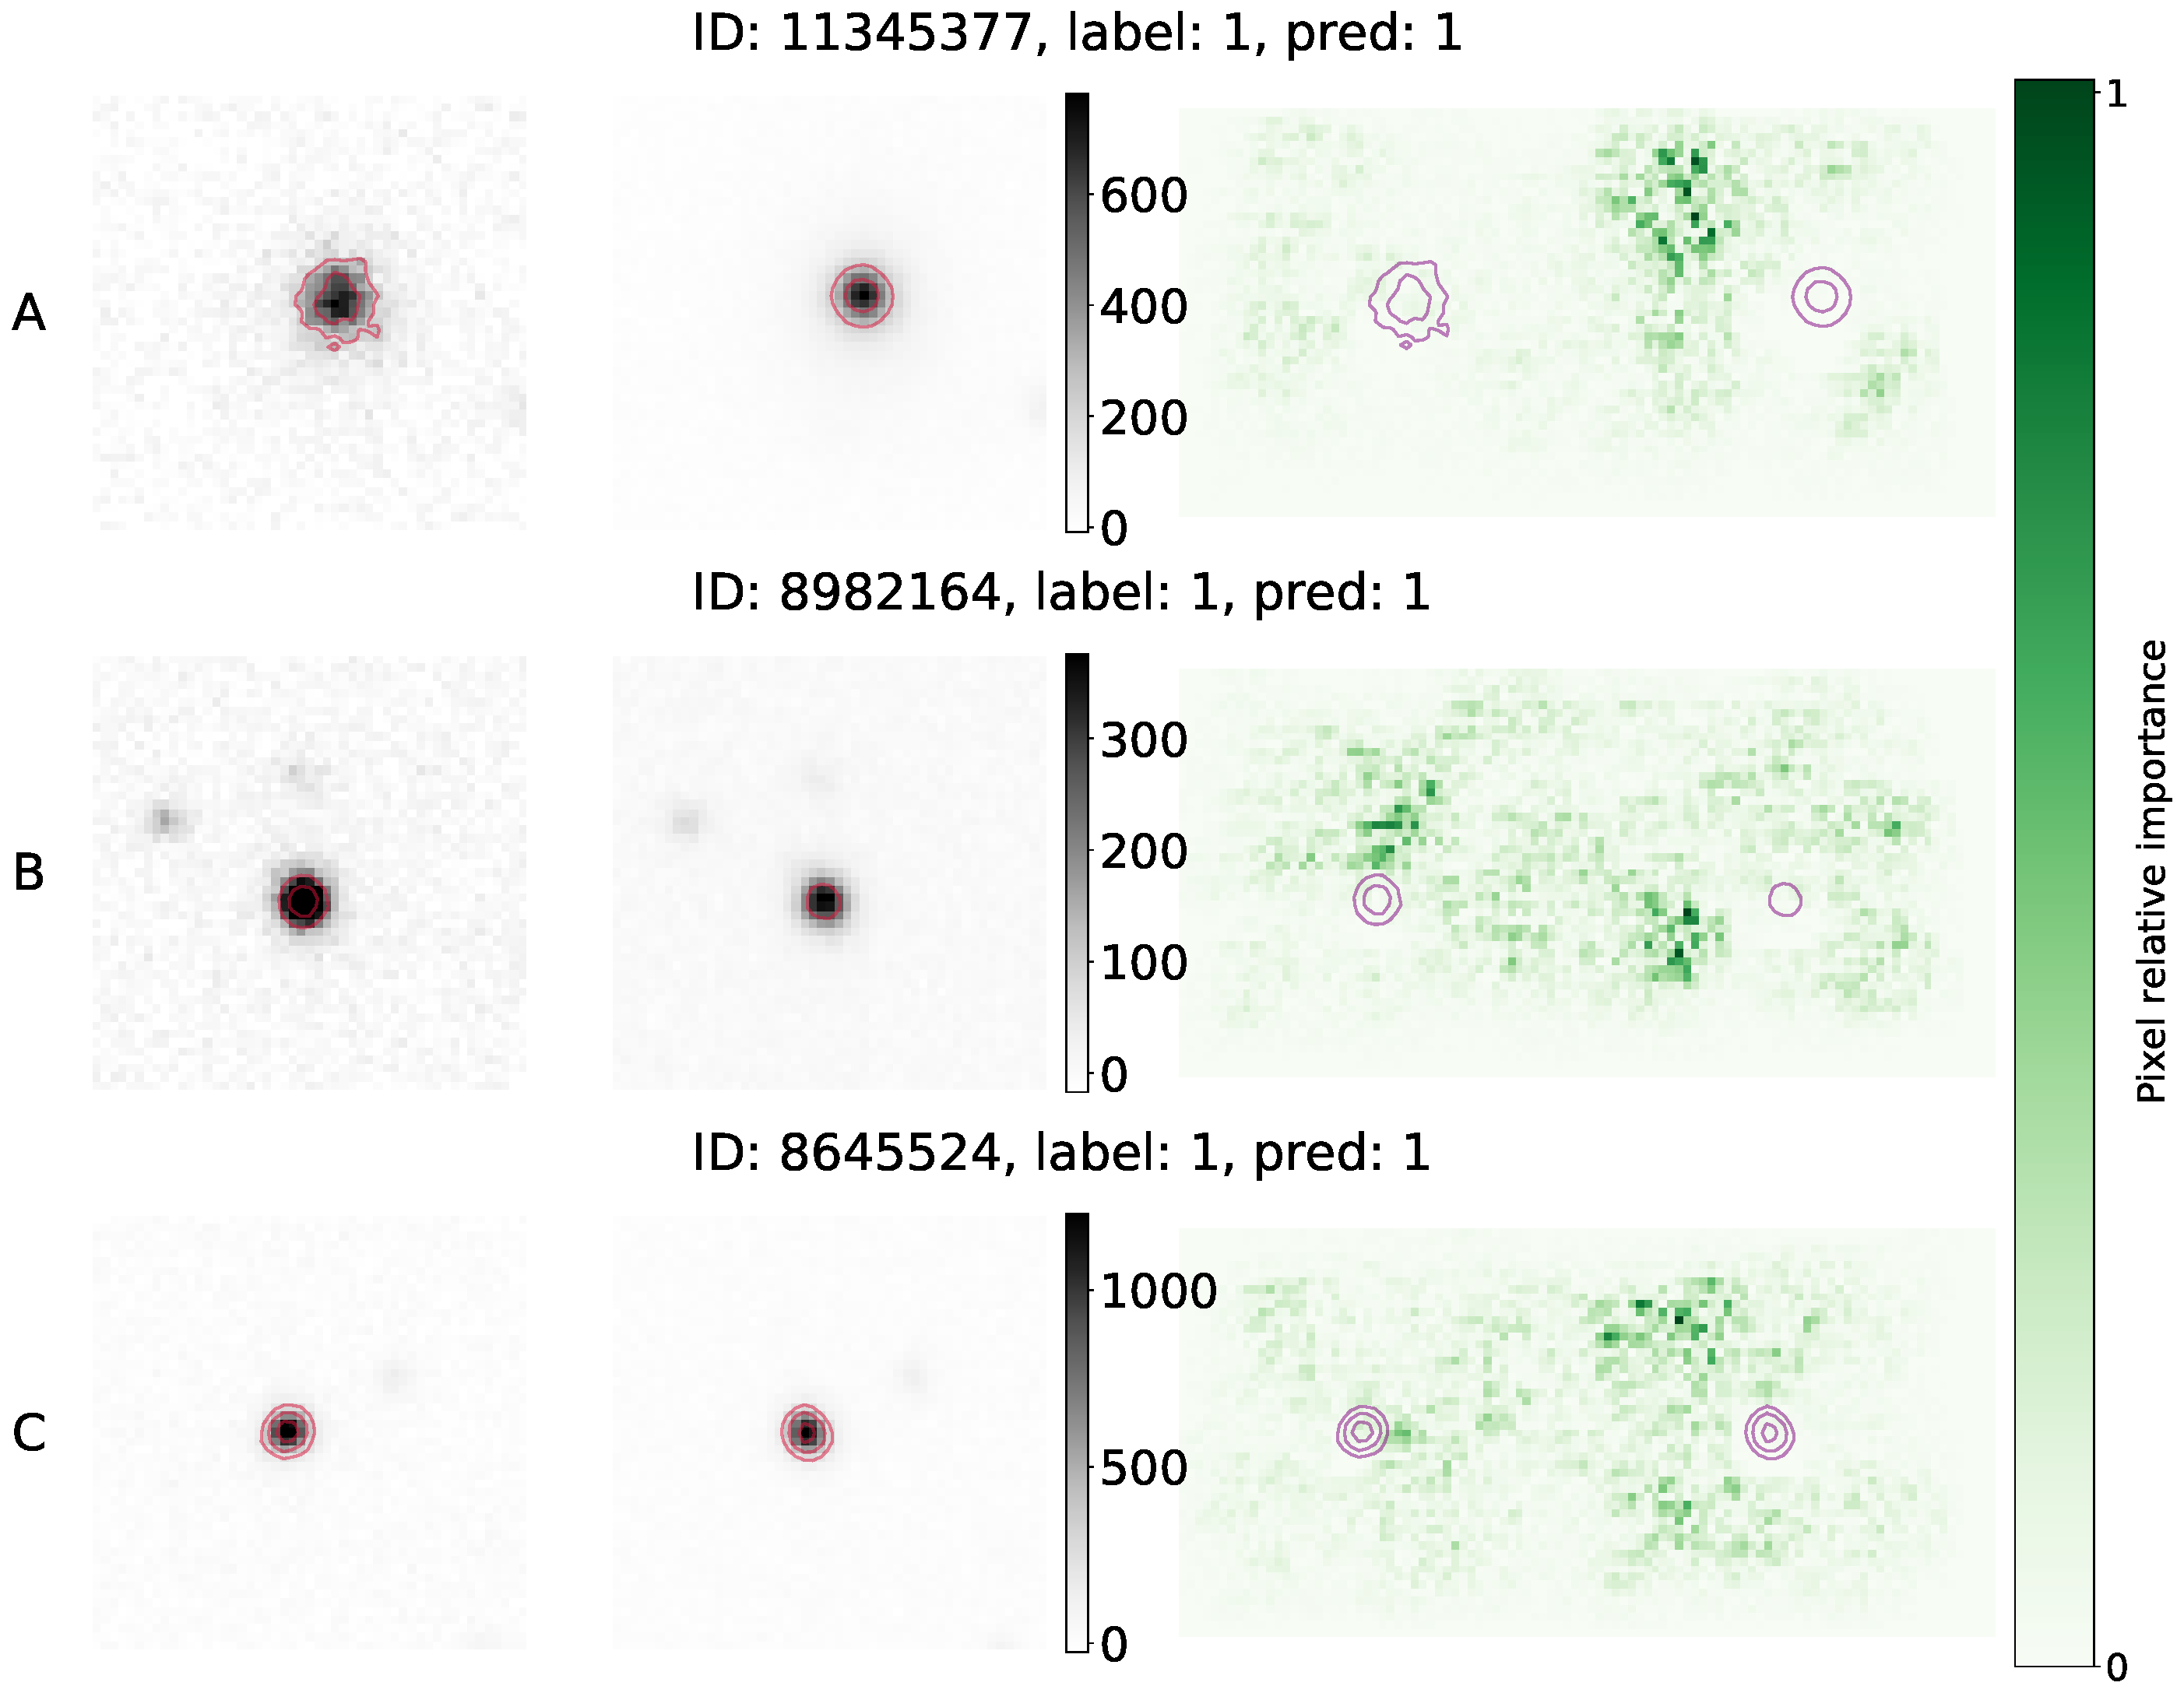
\includegraphics[width=0.65\linewidth]{
    figures/saliency_plot_noDIA3exam.pdf}
    \caption{The same transients (\search-\temp) shown in \autoref{fig:saliency_3id_contour} and their respective saliency maps for \nodia\ model True Negatives (correctly identified ``bogus'').  Important pixels are found at nearly all locations in the image, rather than in a small region around the center. The model needs to learn properties of the image at large to enable a comparison of the \temp\ and \diff.  This figure is further discussed in \hyperref[sec:appendixc]{Appendix C}.}
    \label{fig:saliency_nodia3id_contour}
\end{figure*}


\clearpage
\begin{figure*}
    \centering
    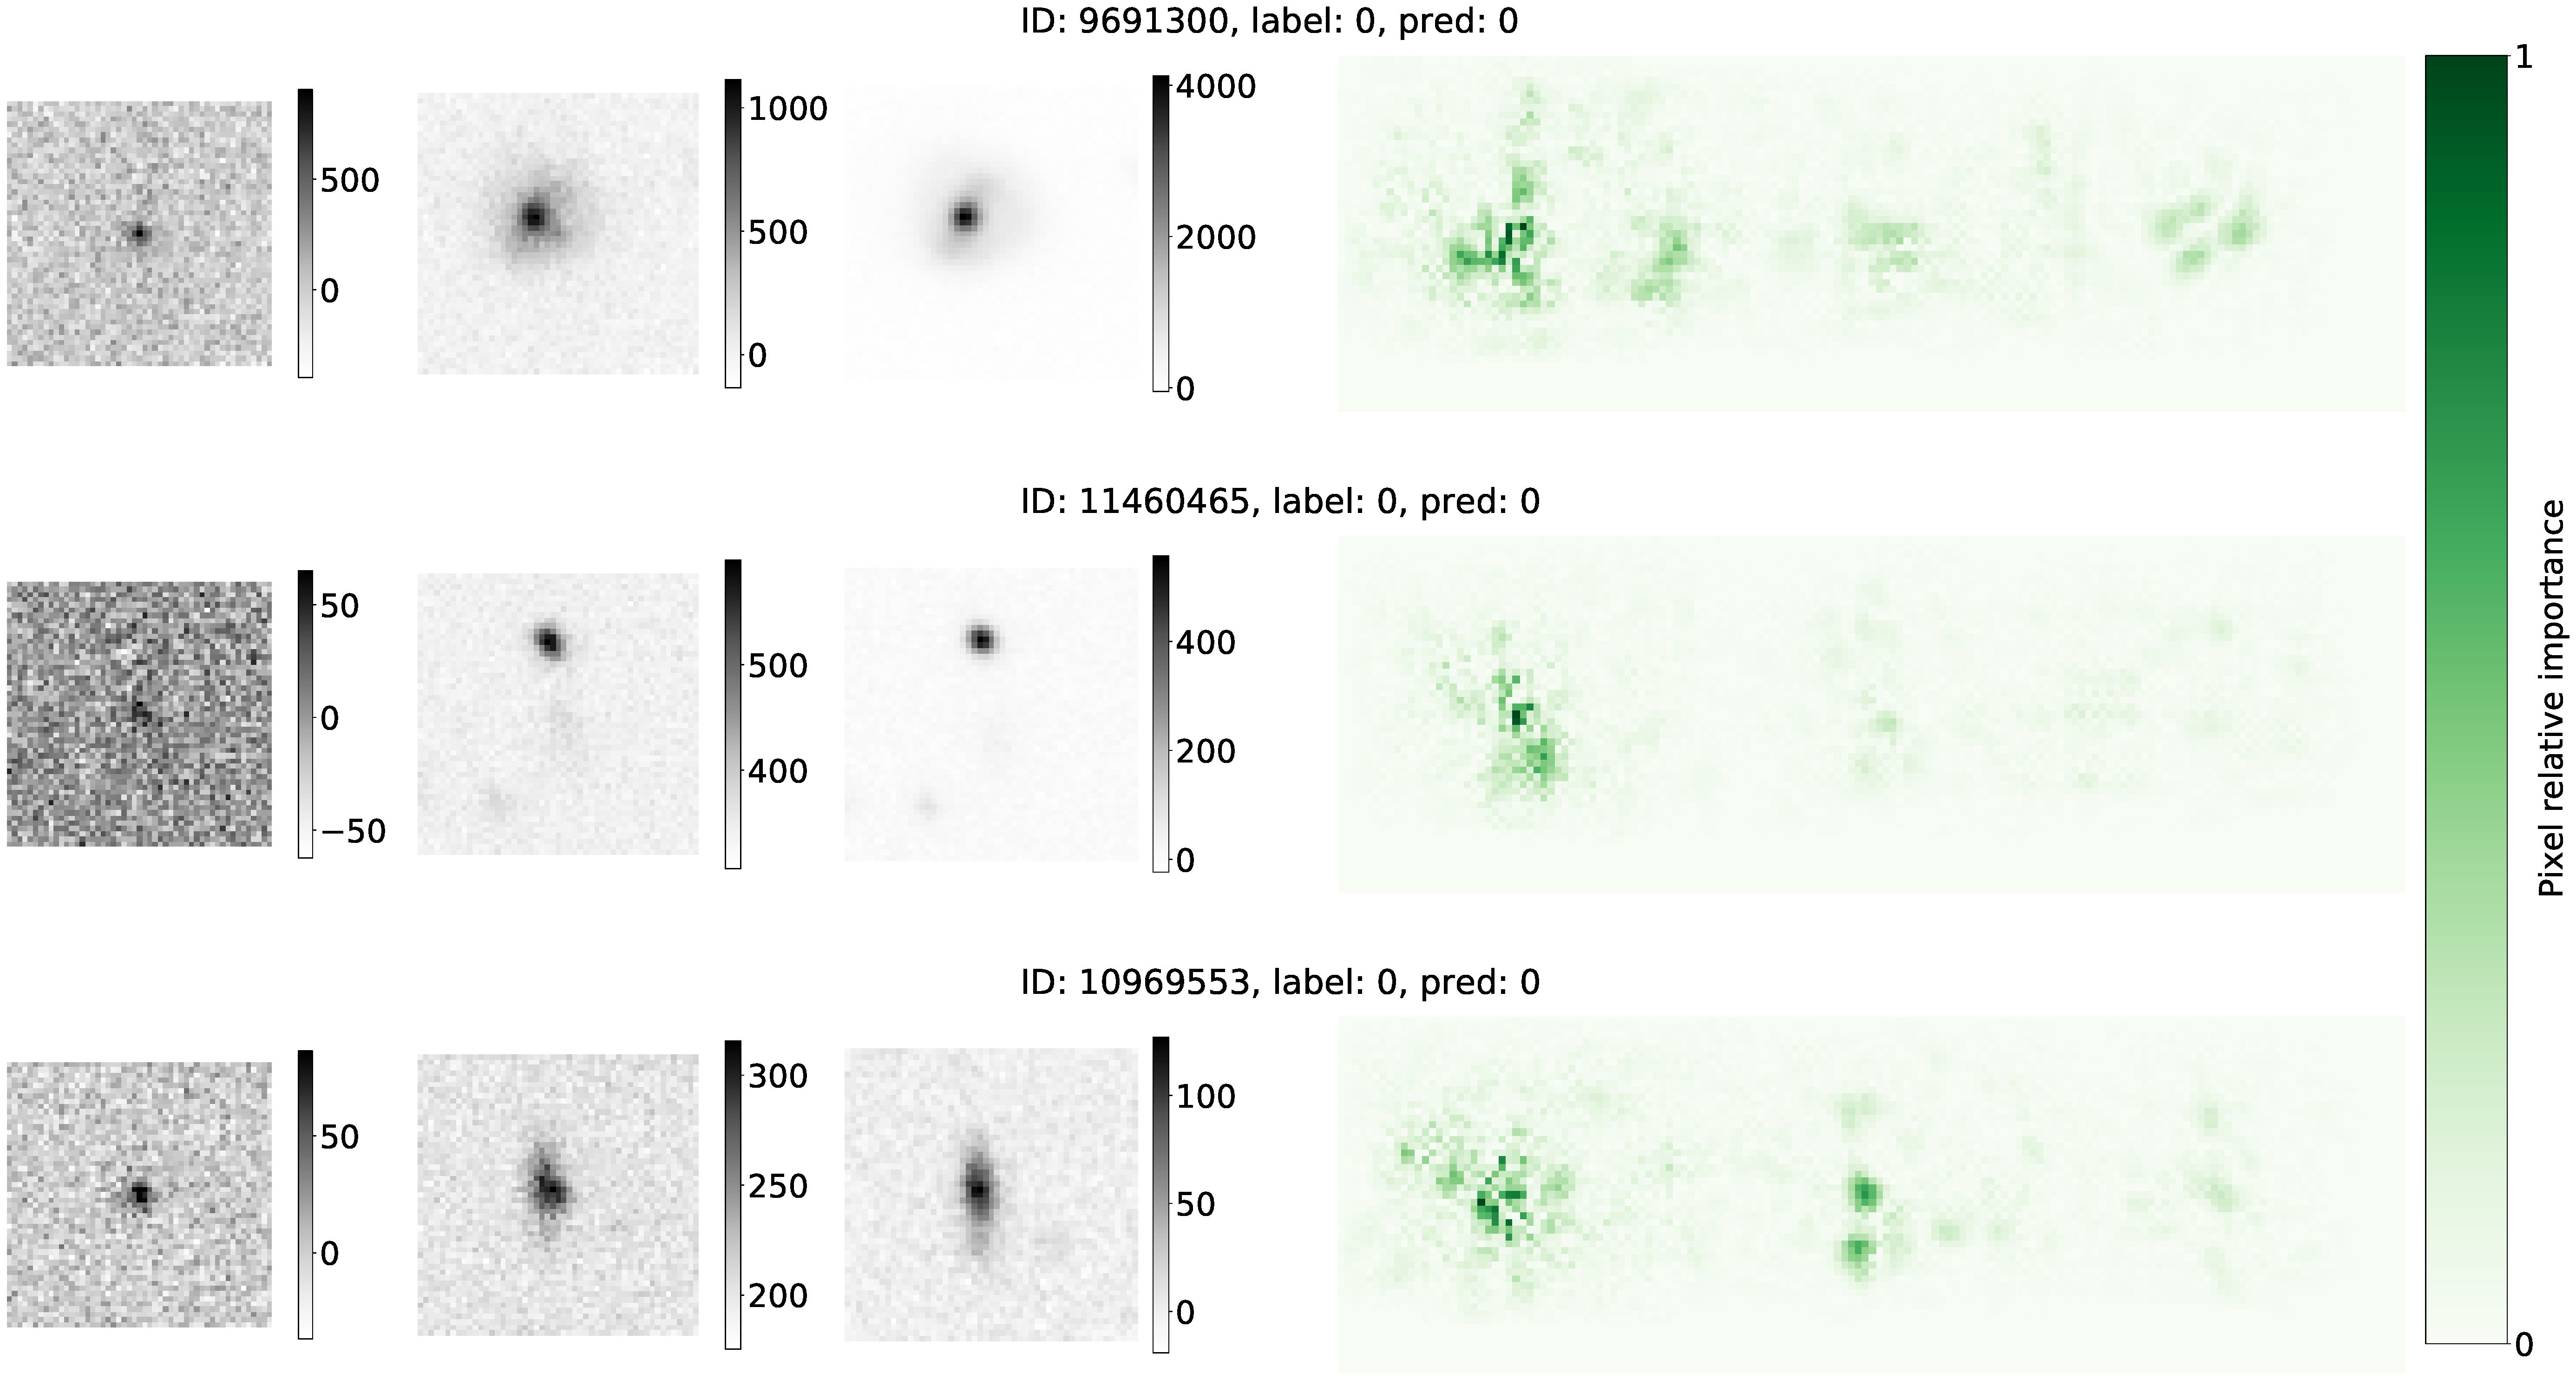
\includegraphics[width=0.8\linewidth]{
    figures/saliency_plot_other3-see64.pdf}
    
    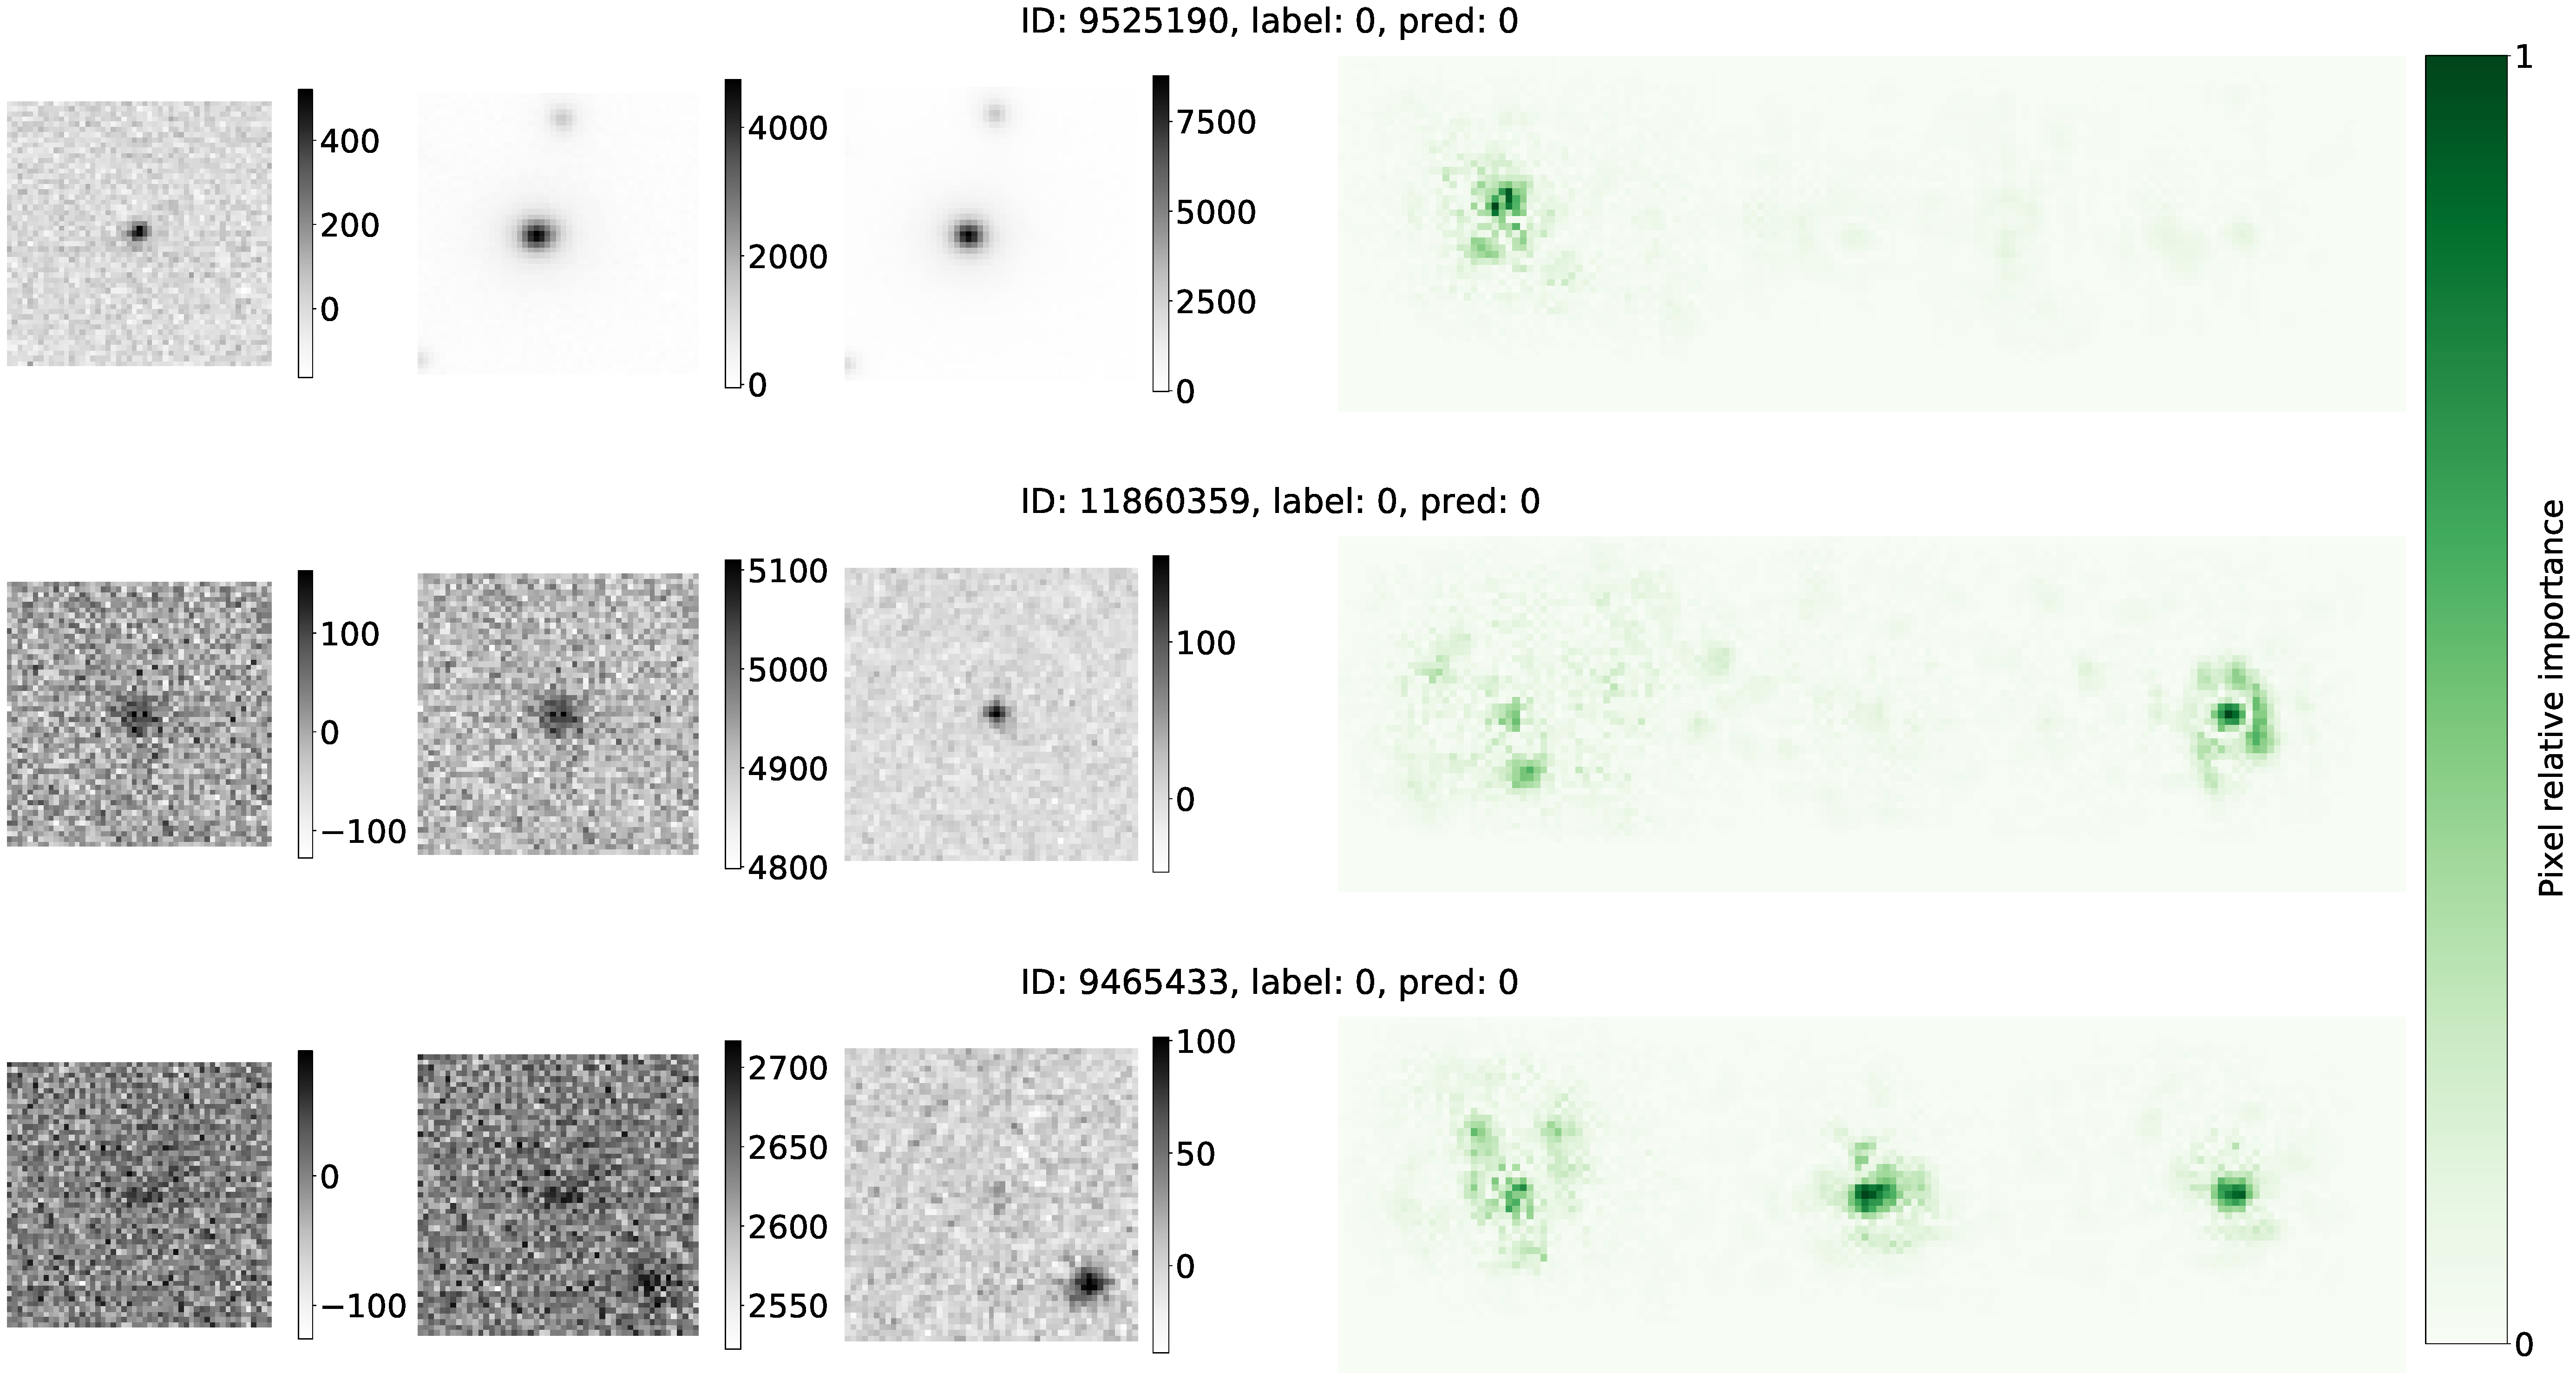
\includegraphics[width=0.8\linewidth]{
    figures/saliency_plot_other3-see109.pdf}
    \caption{Transients (\diff-\search-\temp) and their respective saliency map  for \diabased\ model True Positives  (correctly identified ``real'' astrophysical transients). The important pixels are generally found in the \diff\ portion of the image for the \diabased\ model, as discussed in \autoref{sec:results}, but there are exceptions: here we show several cases of True Positives (real transients) classifications where the component of the image that was principally leveraged by the model was the \diff\ (the leftmost third) but two cases where the \nodia\ relied principally on the \search\ and/or \temp\ (bottom two panels).}
    \label{fig:saliency_dia3id_TP}
\end{figure*}


\begin{figure*}
    \centering
    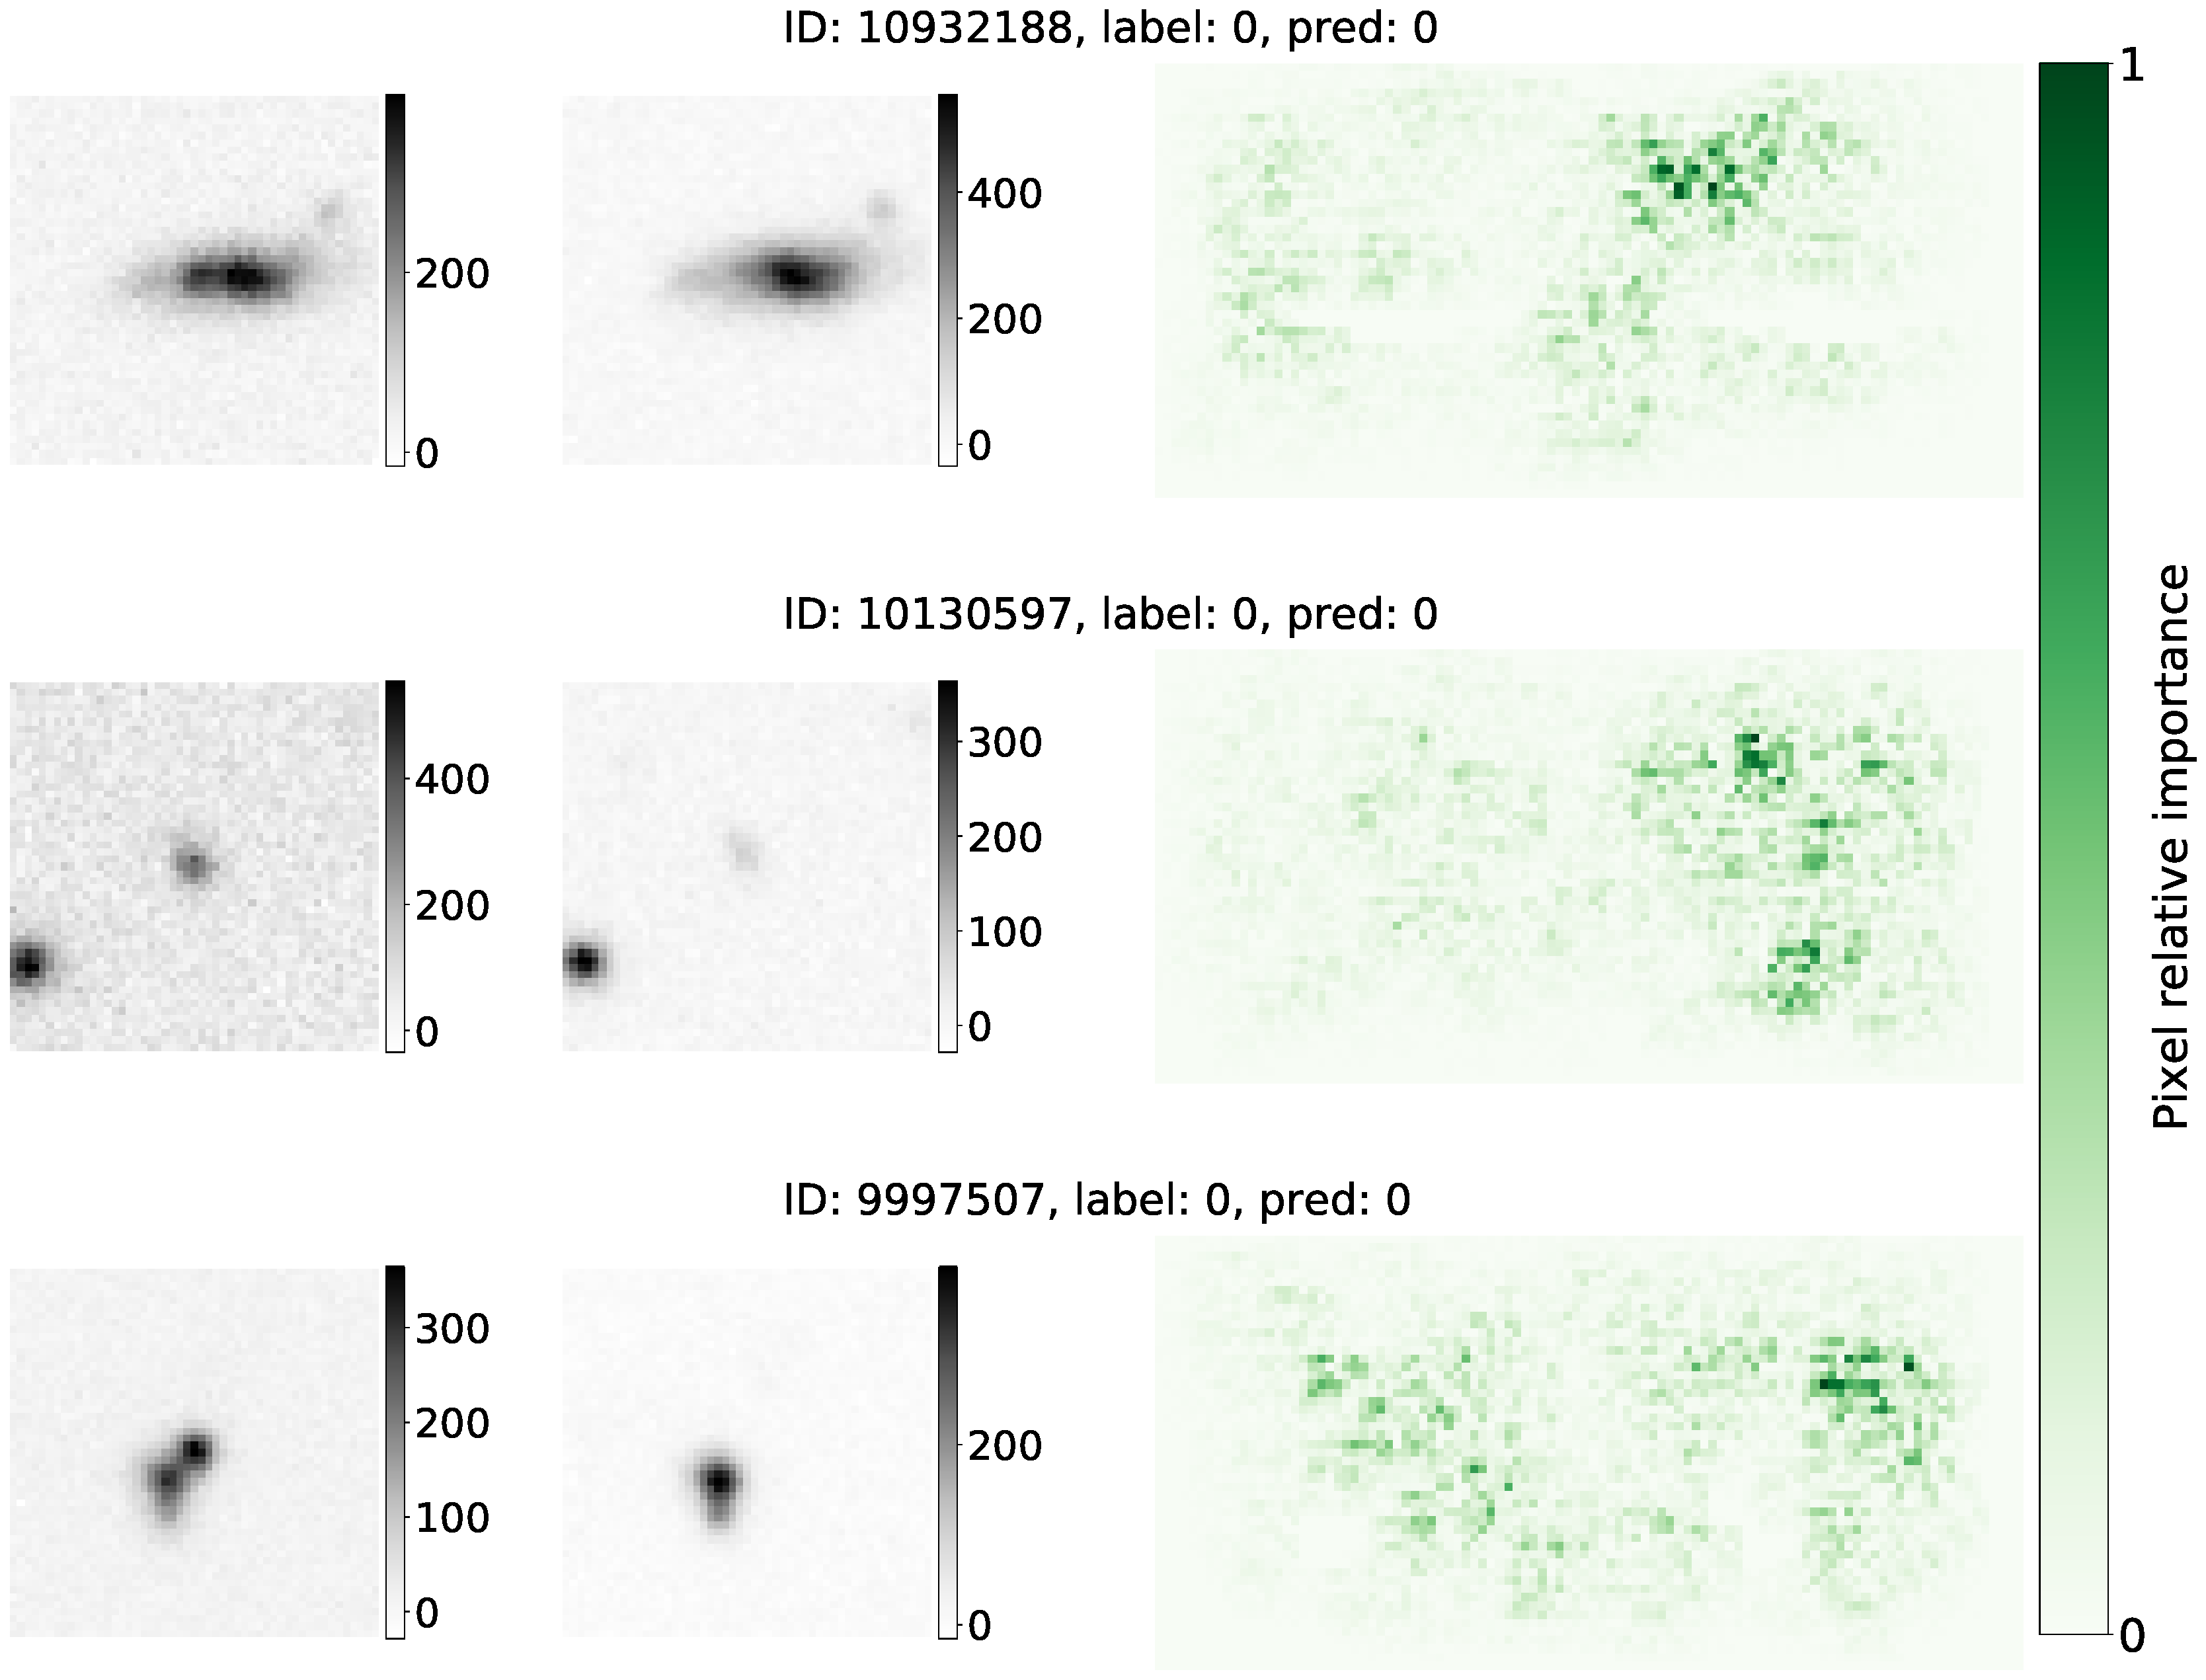
\includegraphics[width=0.8\linewidth]{
    figures/saliency_plot_other3nodiaTP-see766.pdf}
    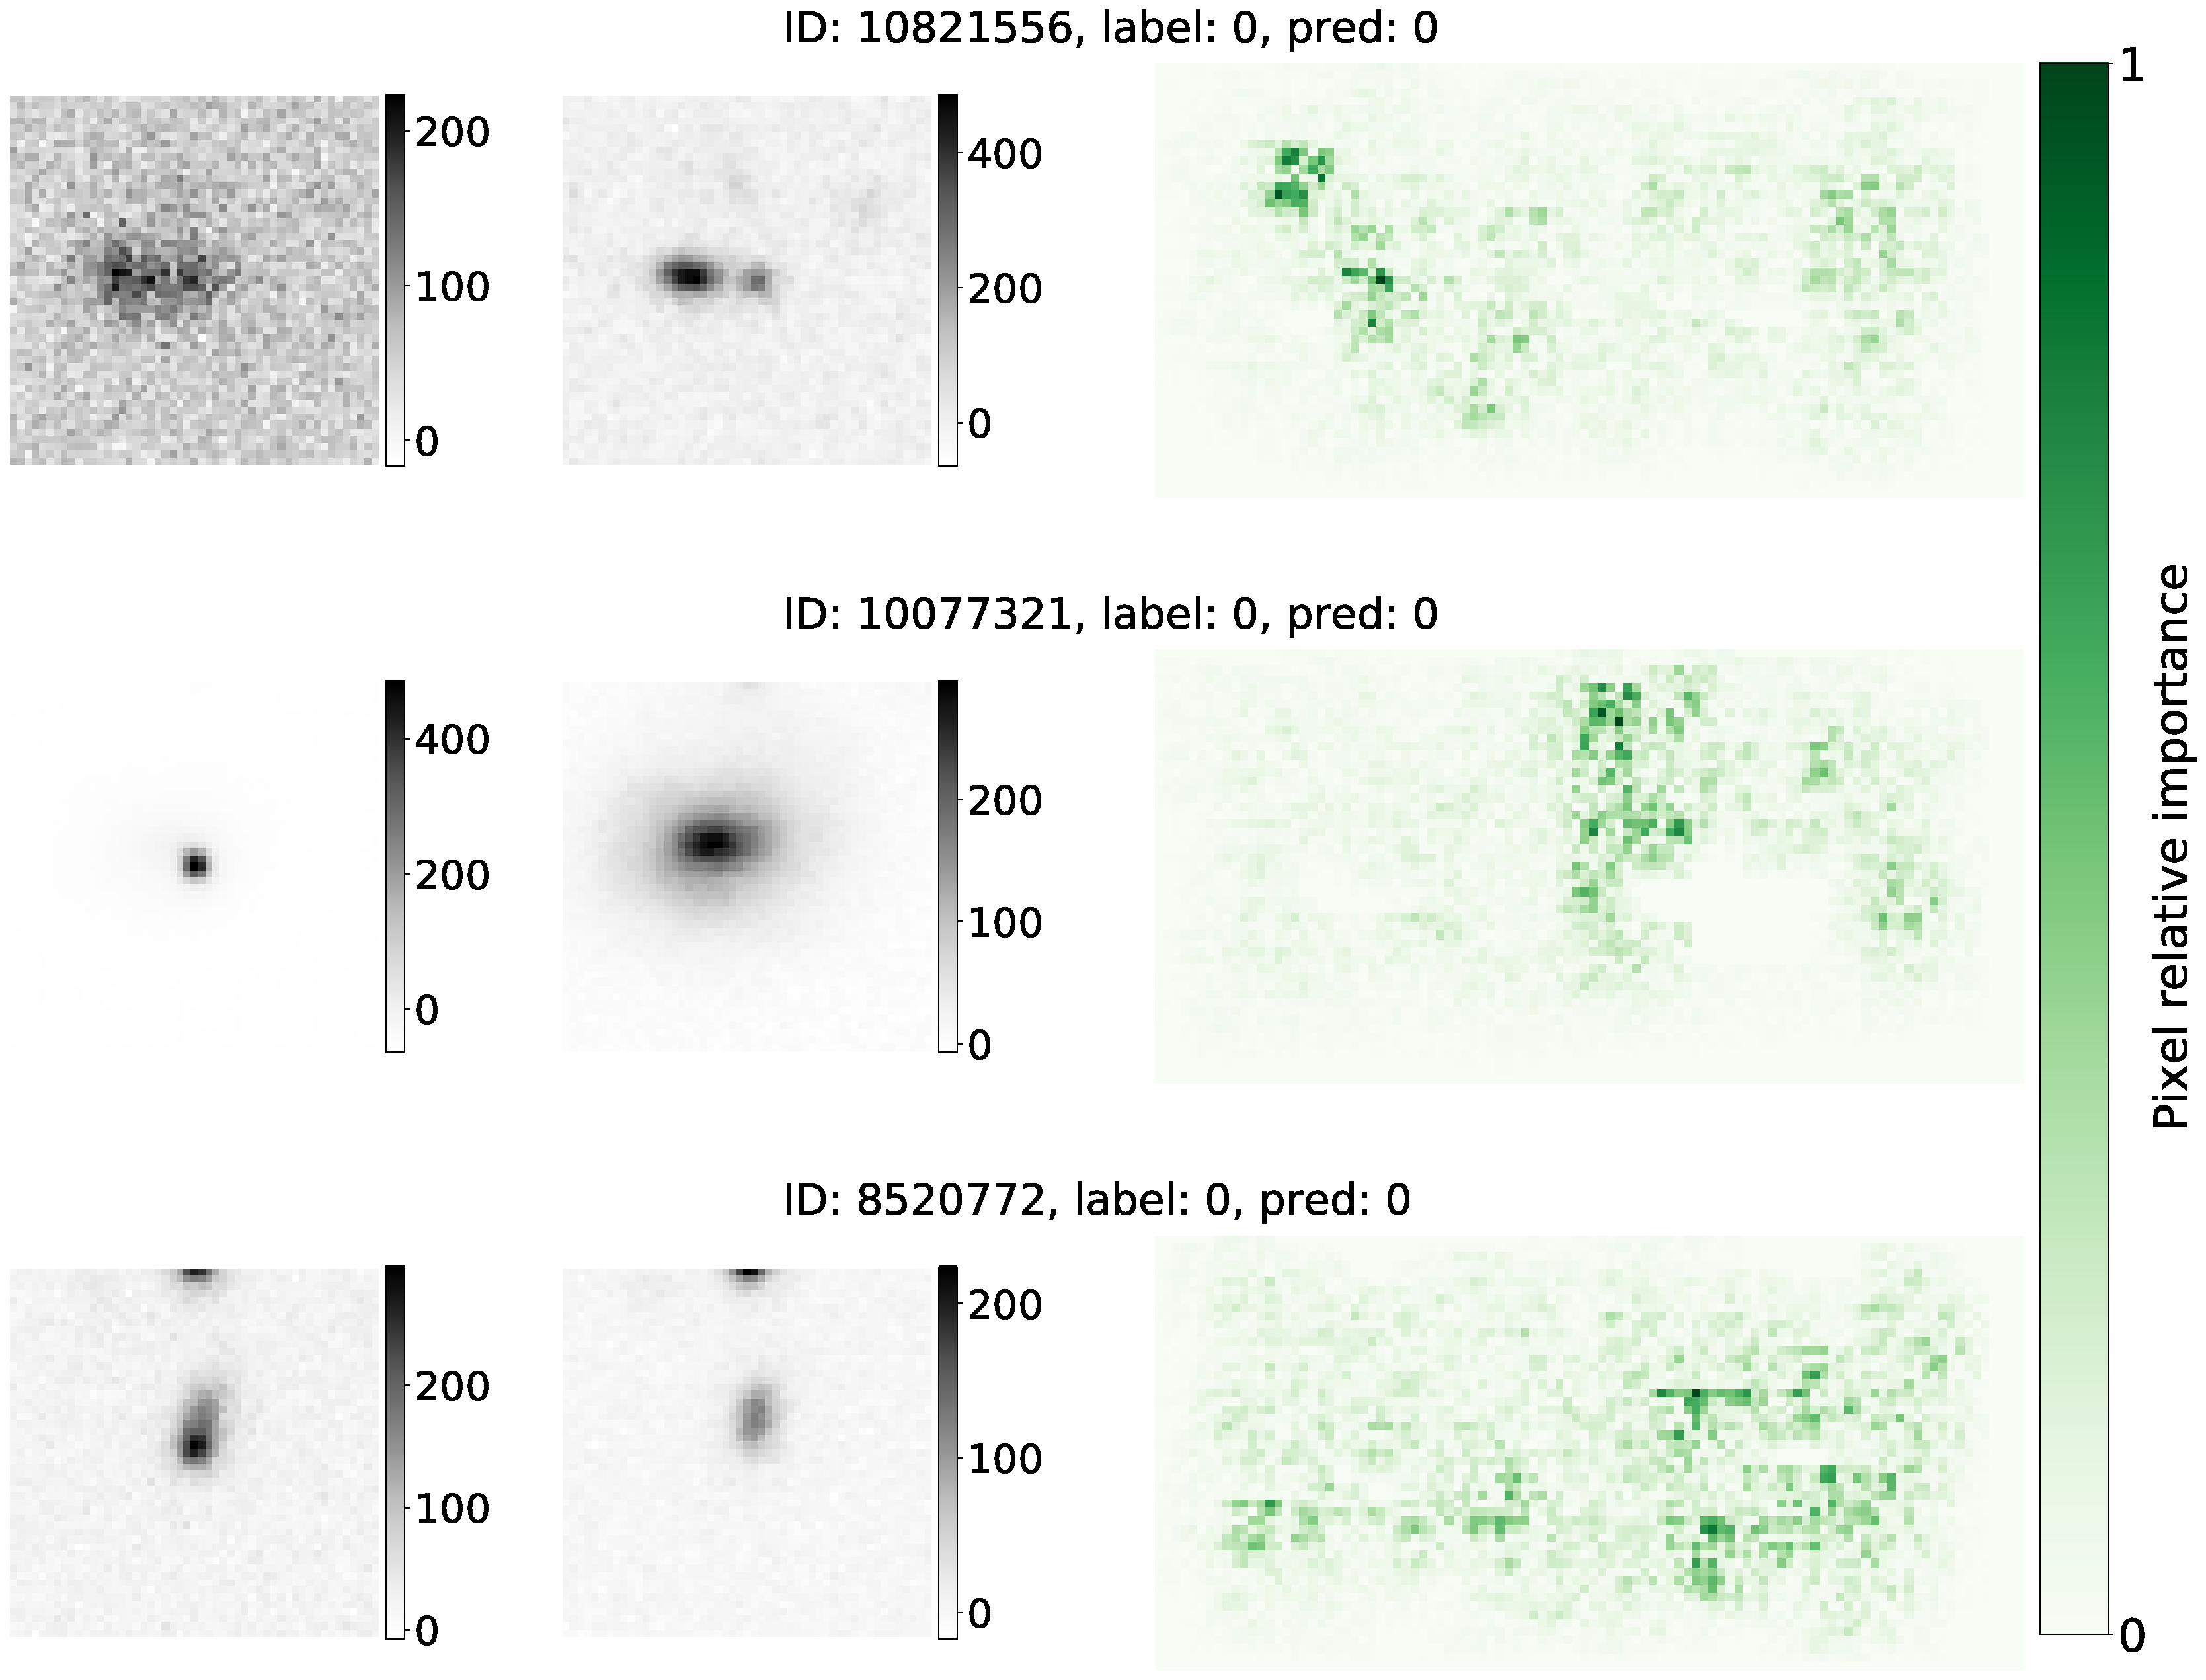
\includegraphics[width=0.8\linewidth]{
    figures/saliency_plot_other3nodiaTP-see7407.pdf}
   \caption{Transients (\search-\temp) and their respective saliency map for the \nodia\ model True Positives  (correctly identified ``real'' astrophysical transients). Important pixels are found everywhere in the image, as the CNN learns how to compare the \diff\ and \temp\ taking a synoptic look at the properties of each image component.}
    \label{fig:tpndia}
\end{figure*}

\begin{figure*}
    \centering
    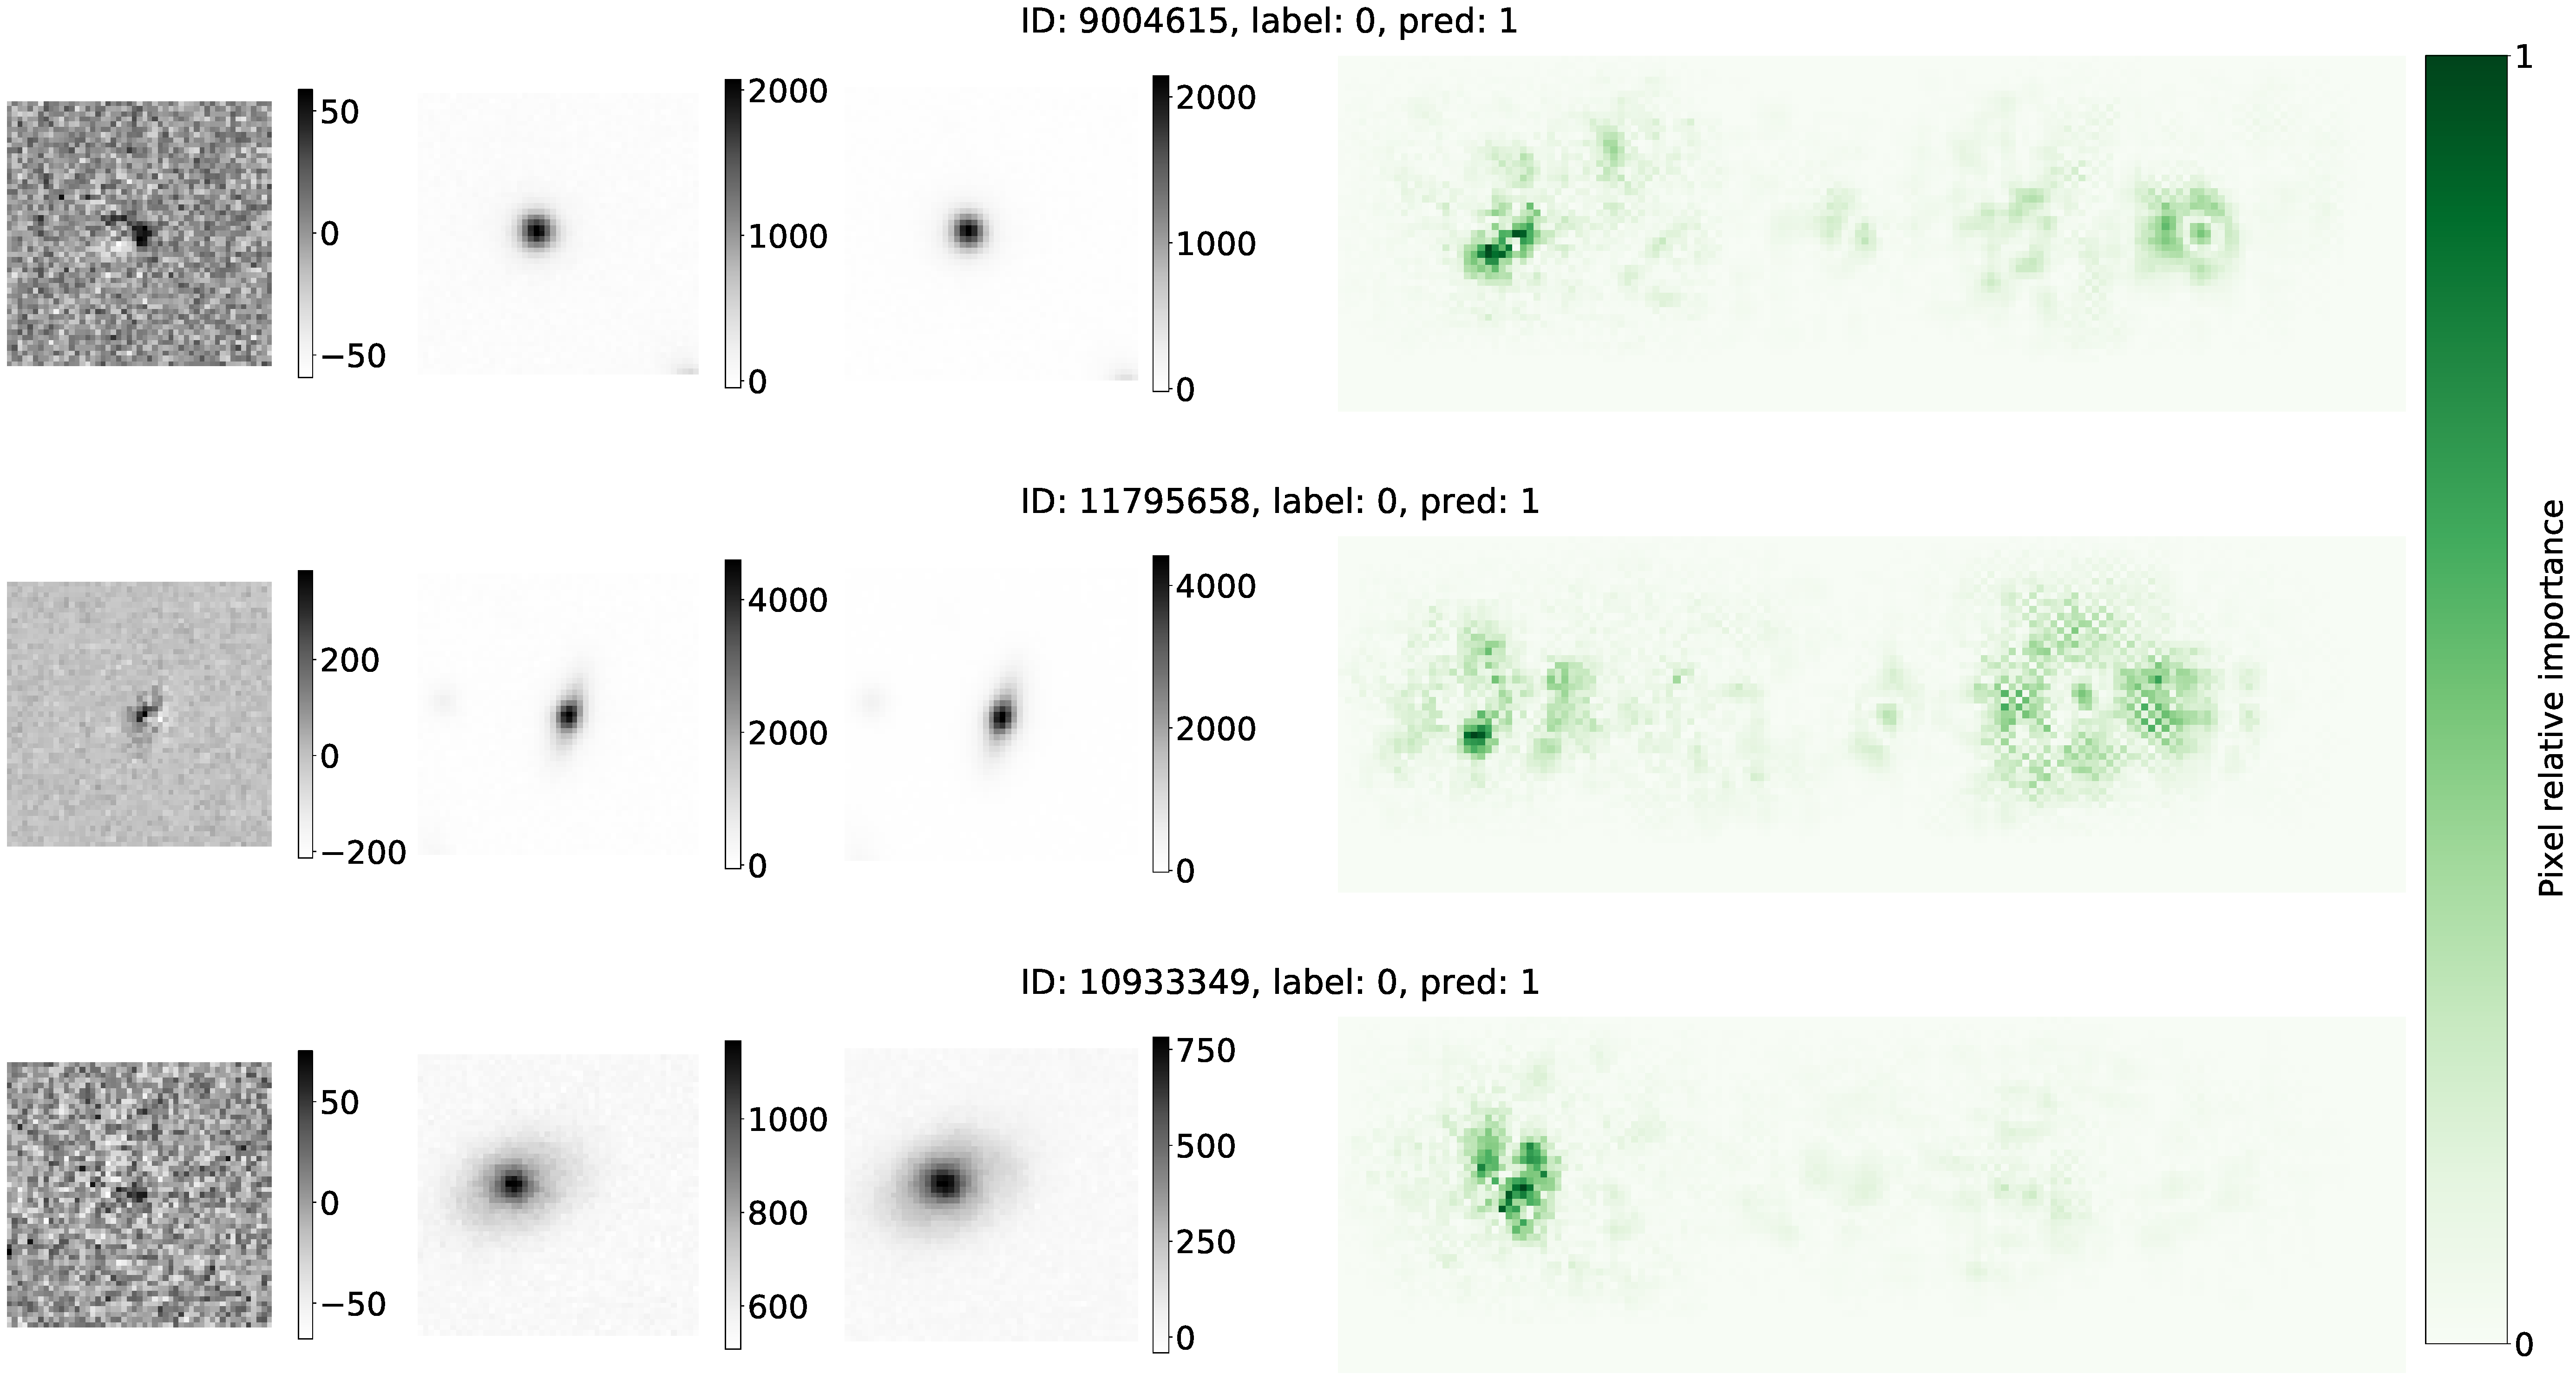
\includegraphics[width=0.8\linewidth]{
    figures/saliency_plot_other3FN-see66.pdf}
    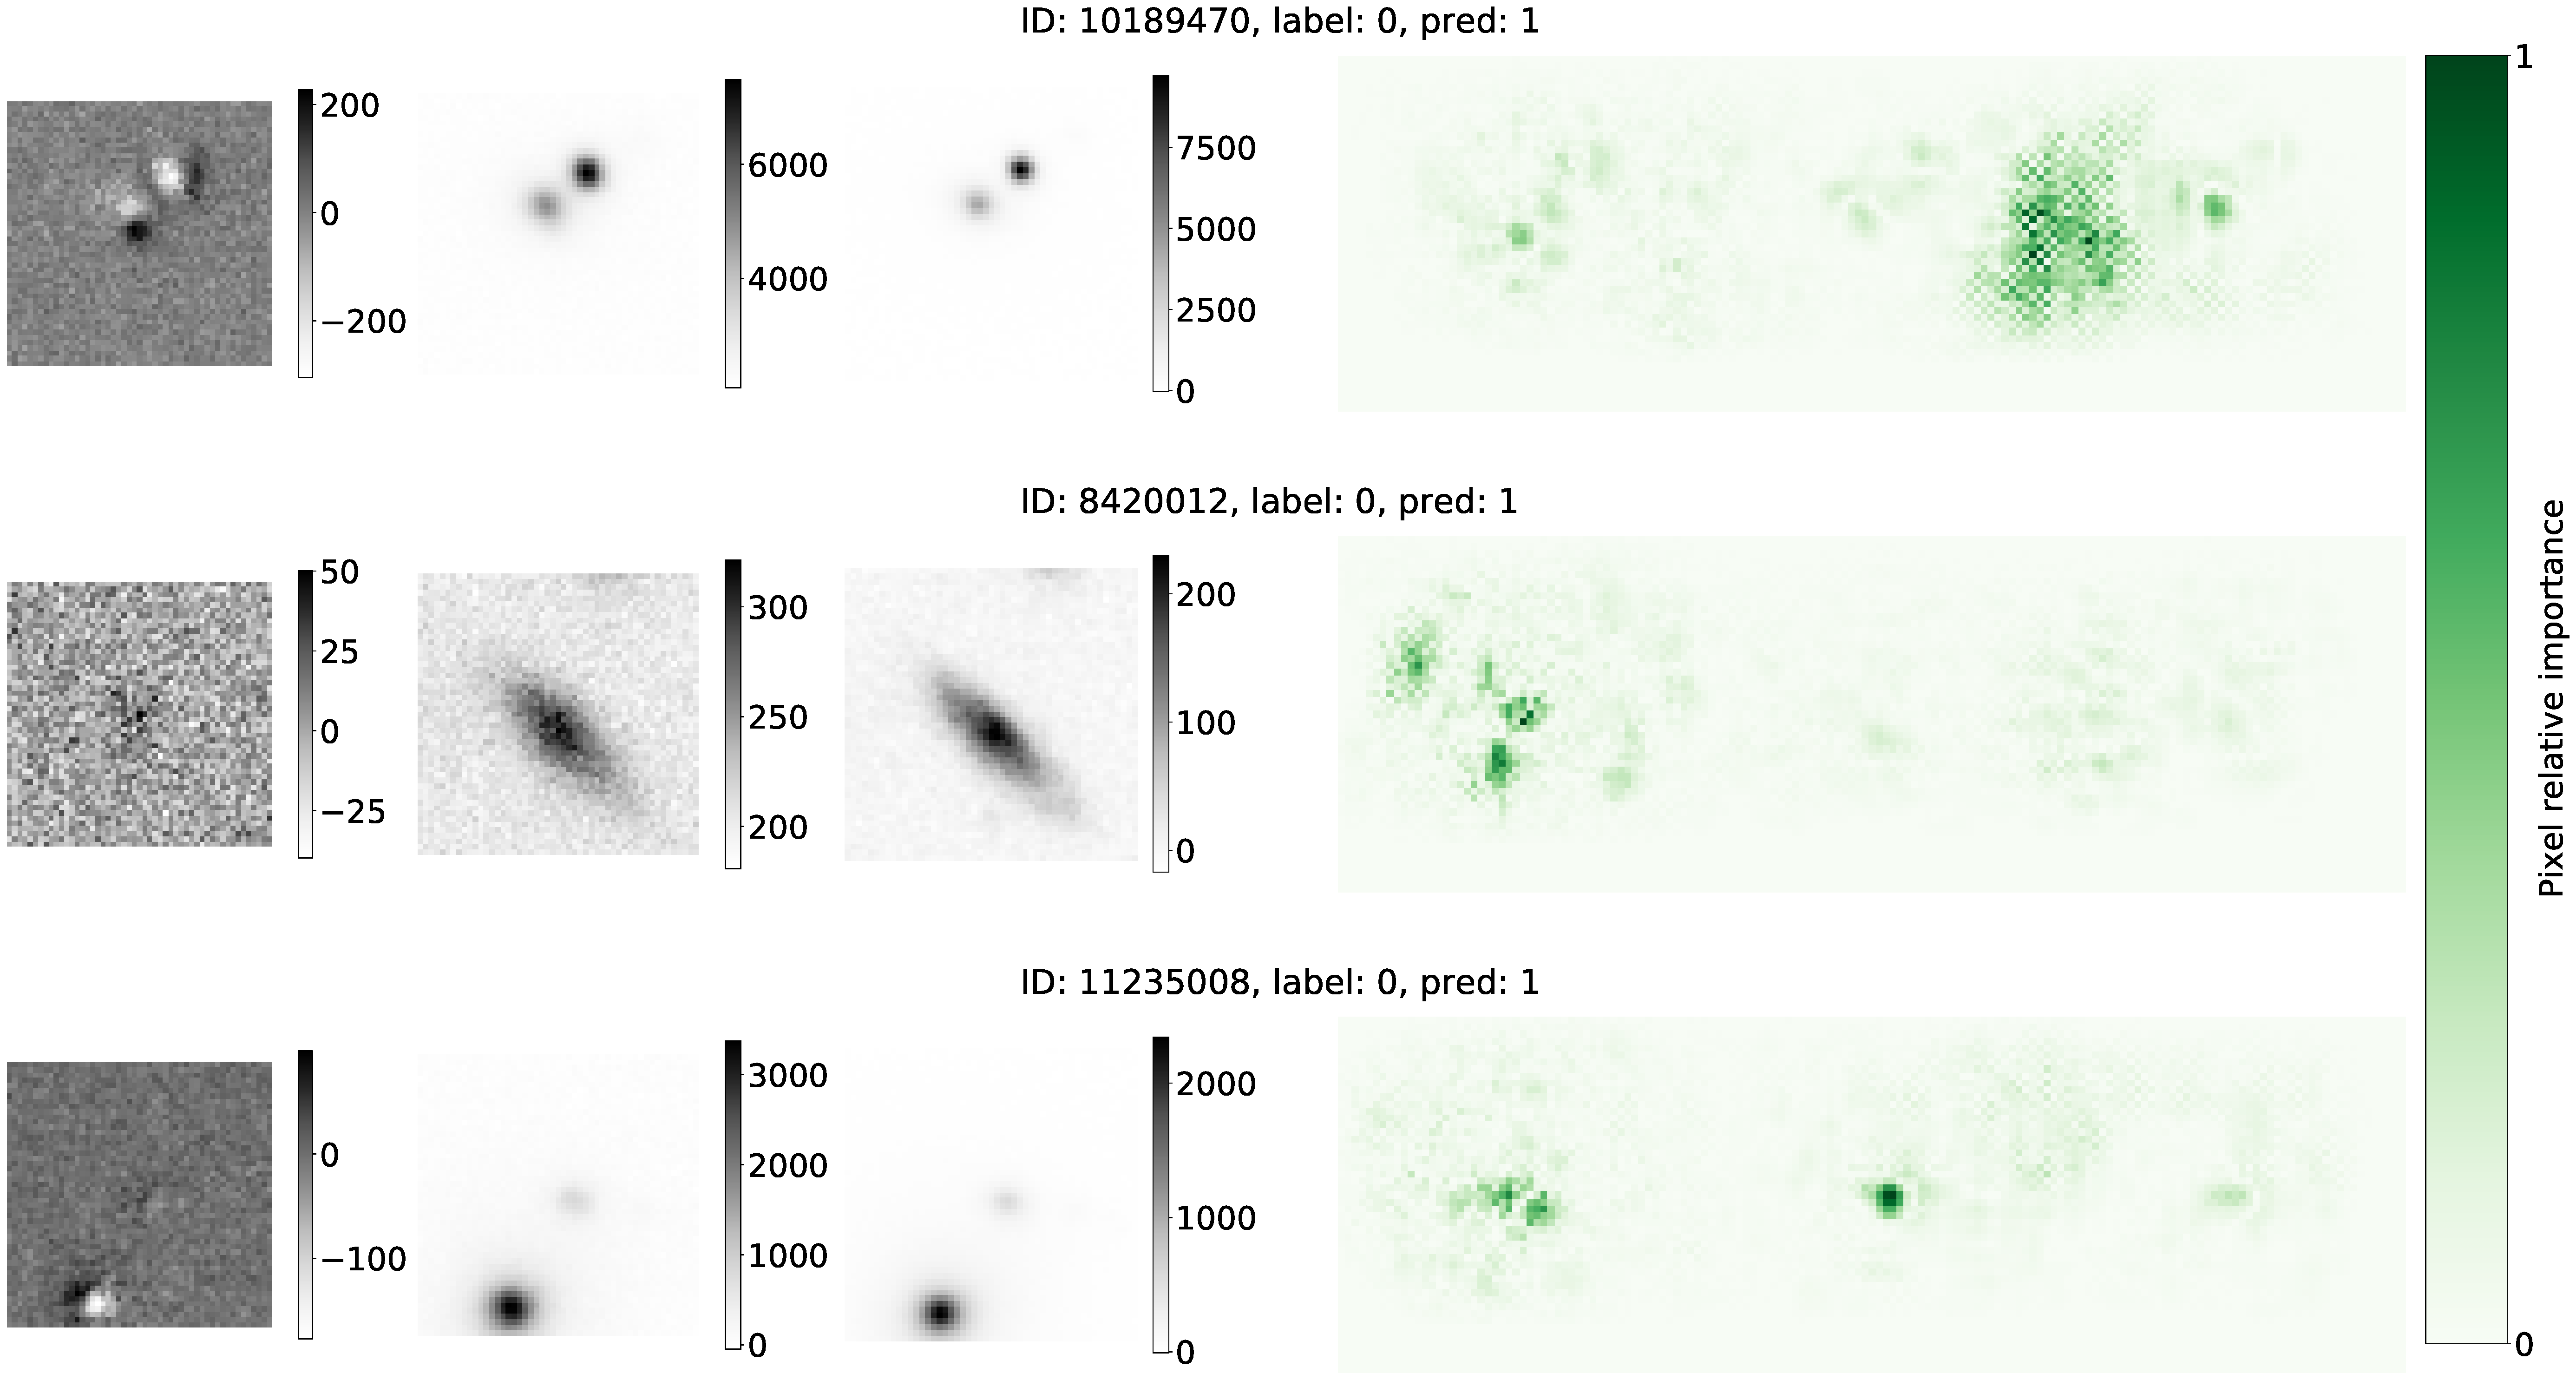
\includegraphics[width=0.8\linewidth]{
    figures/saliency_plot_other3FN-see2041.pdf}
    \caption{Transients (\diff-\search-\temp)  and their respective saliency map for \diabased\ model False Negatives (real transients identified as ``bogus'').
    We remind the reader that the labels are inherited from  \citet{Goldstein_2015} and cannot be verified. Some level of label inaccuracy is expected. The ``real'' transients in this dataset are implanted supernovae onto real DES images. However, in this collection, several transient display DIA inaccuracies (row 1, 2, 4, 6 show ``dipoles'', see \autoref{sec:DI}) that likely lead to the incorrect classification. Two very low signal-to-noise detections are missed (row 3 and 5) by our model.
    Important pixels are more commonly found in \diff\ portion of the image. In the \search\ saliency maps we see again that the core of the central source is used in the classification, as well as pixels that surround the source, but these two sets of important pixels are separate by it by a gap, again reminiscent of the typical aperture photometry technique (top two panels). } 
    \label{fig:saliency_dia3id_FN}
\end{figure*}




\begin{figure*}
    \centering
    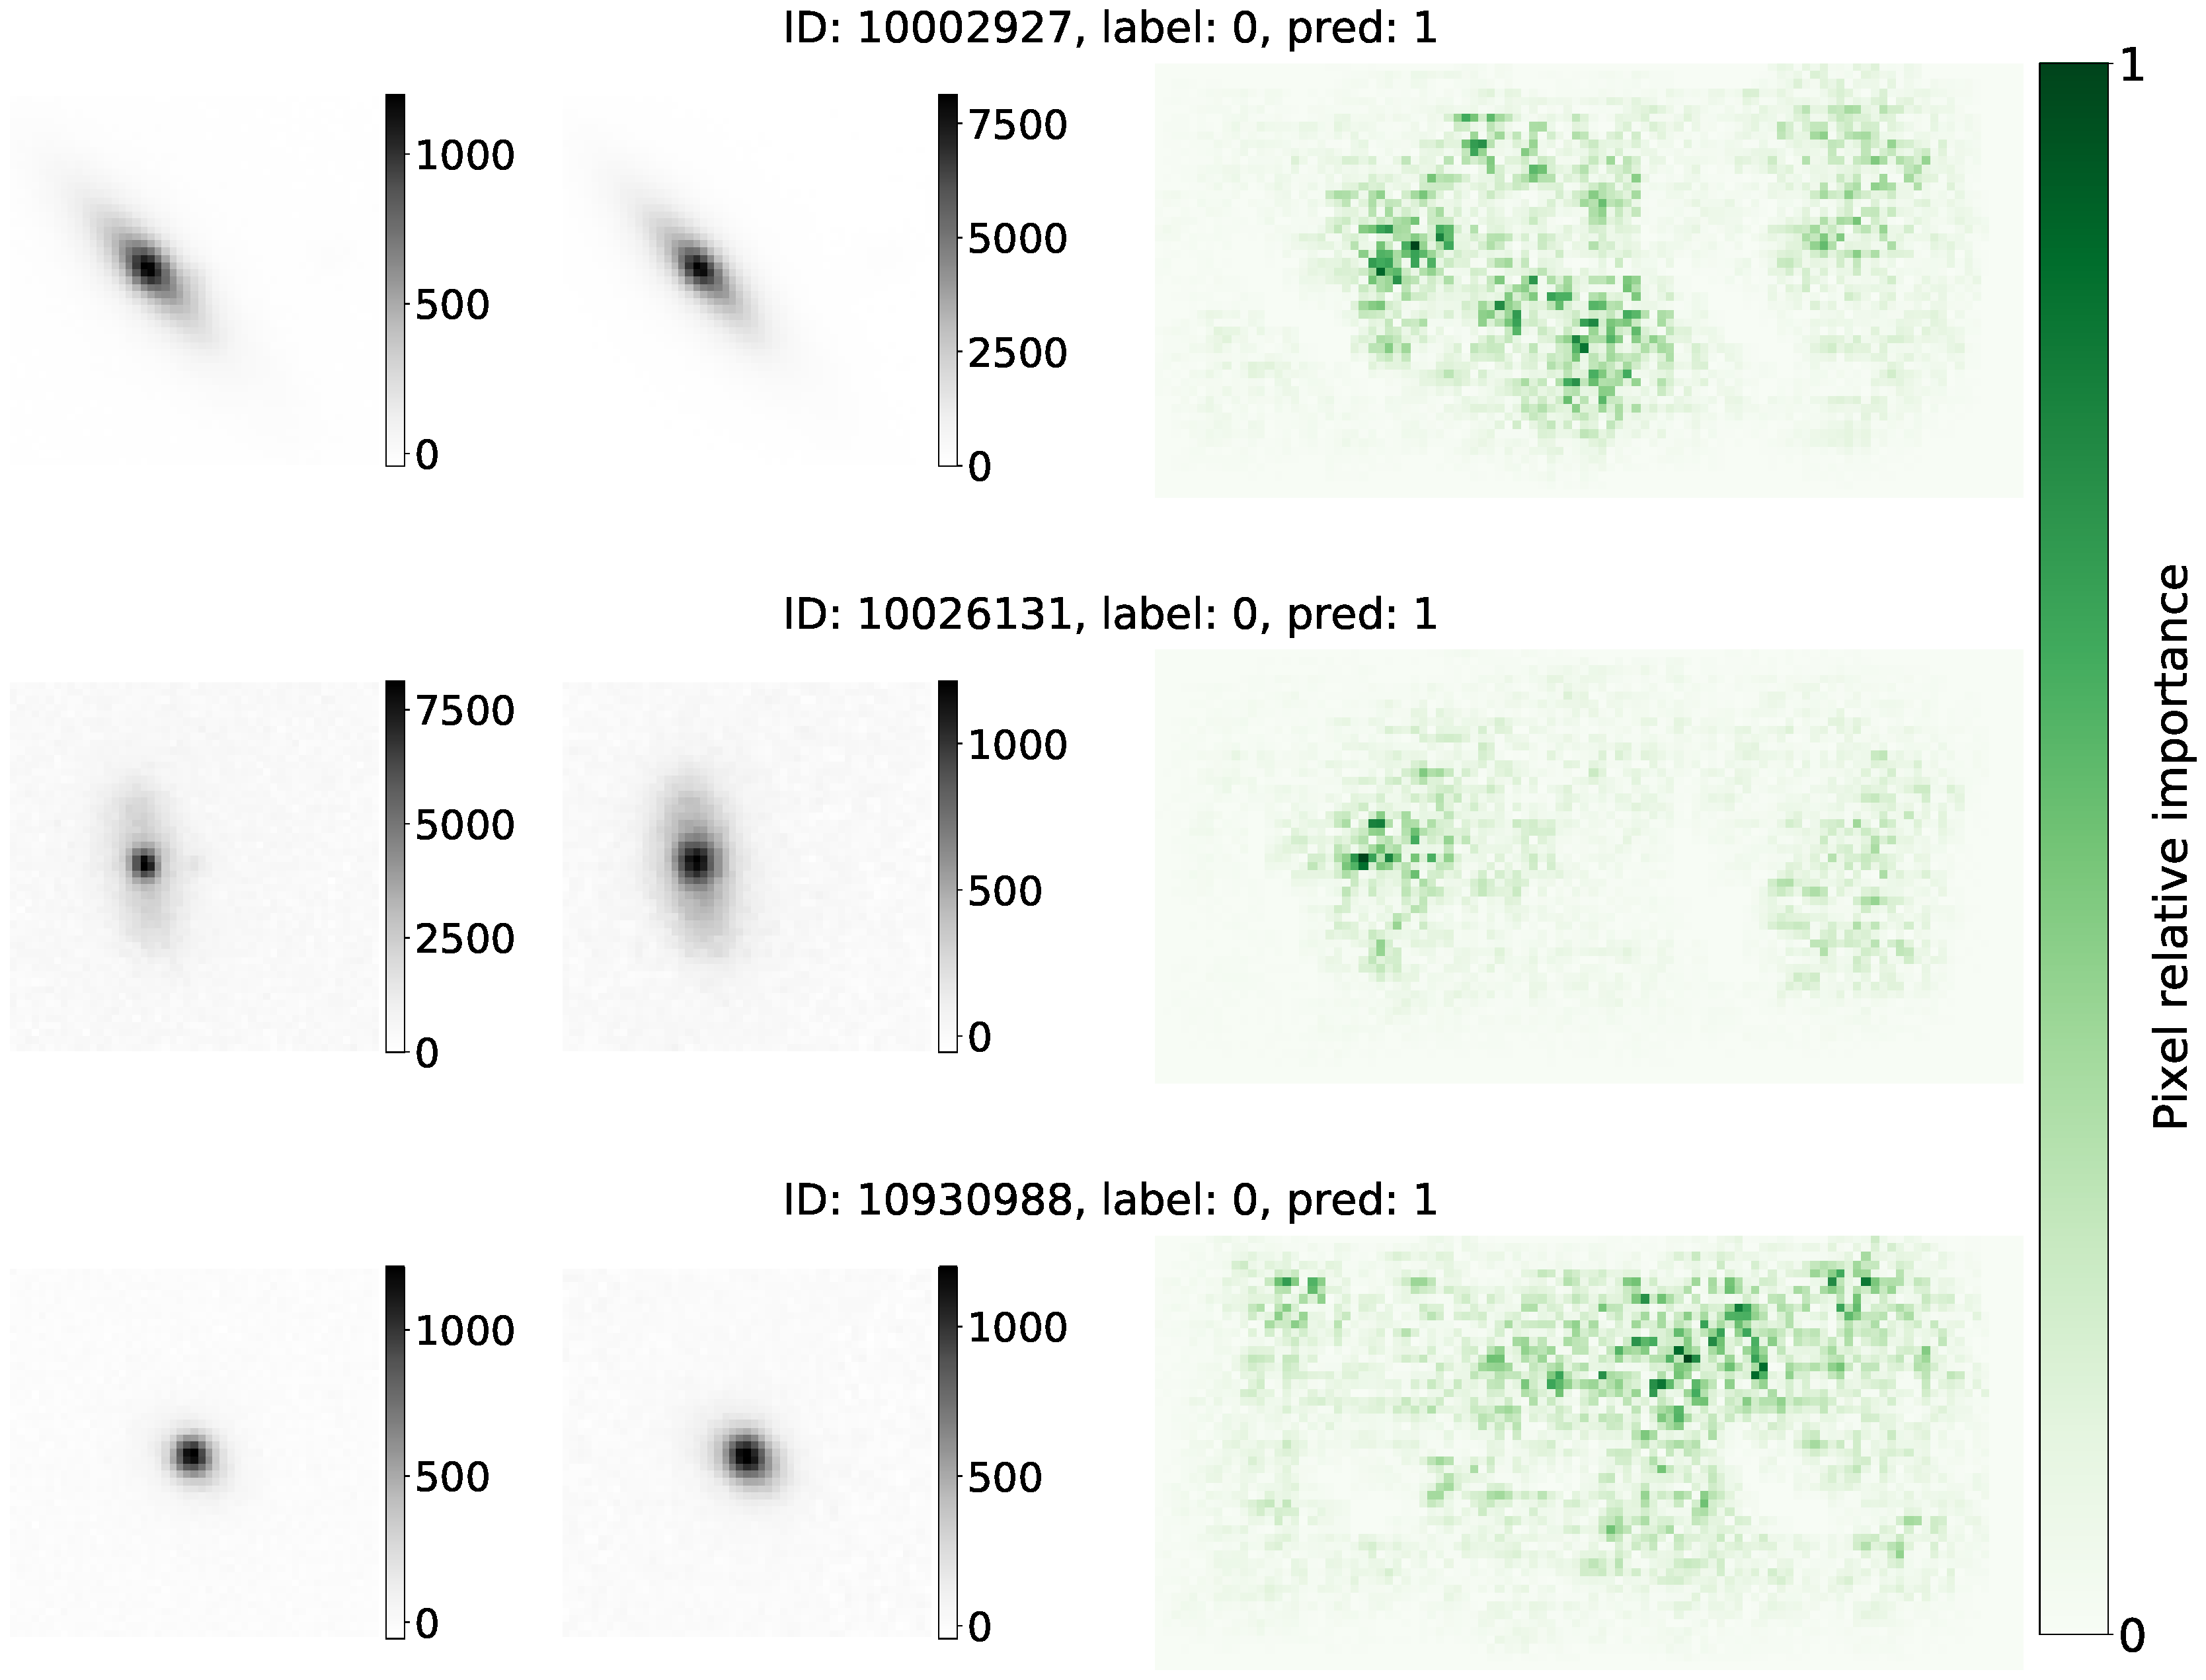
\includegraphics[width=0.76\linewidth]{
    figures/saliency_plot_other3nodiaFN-see356.pdf}
    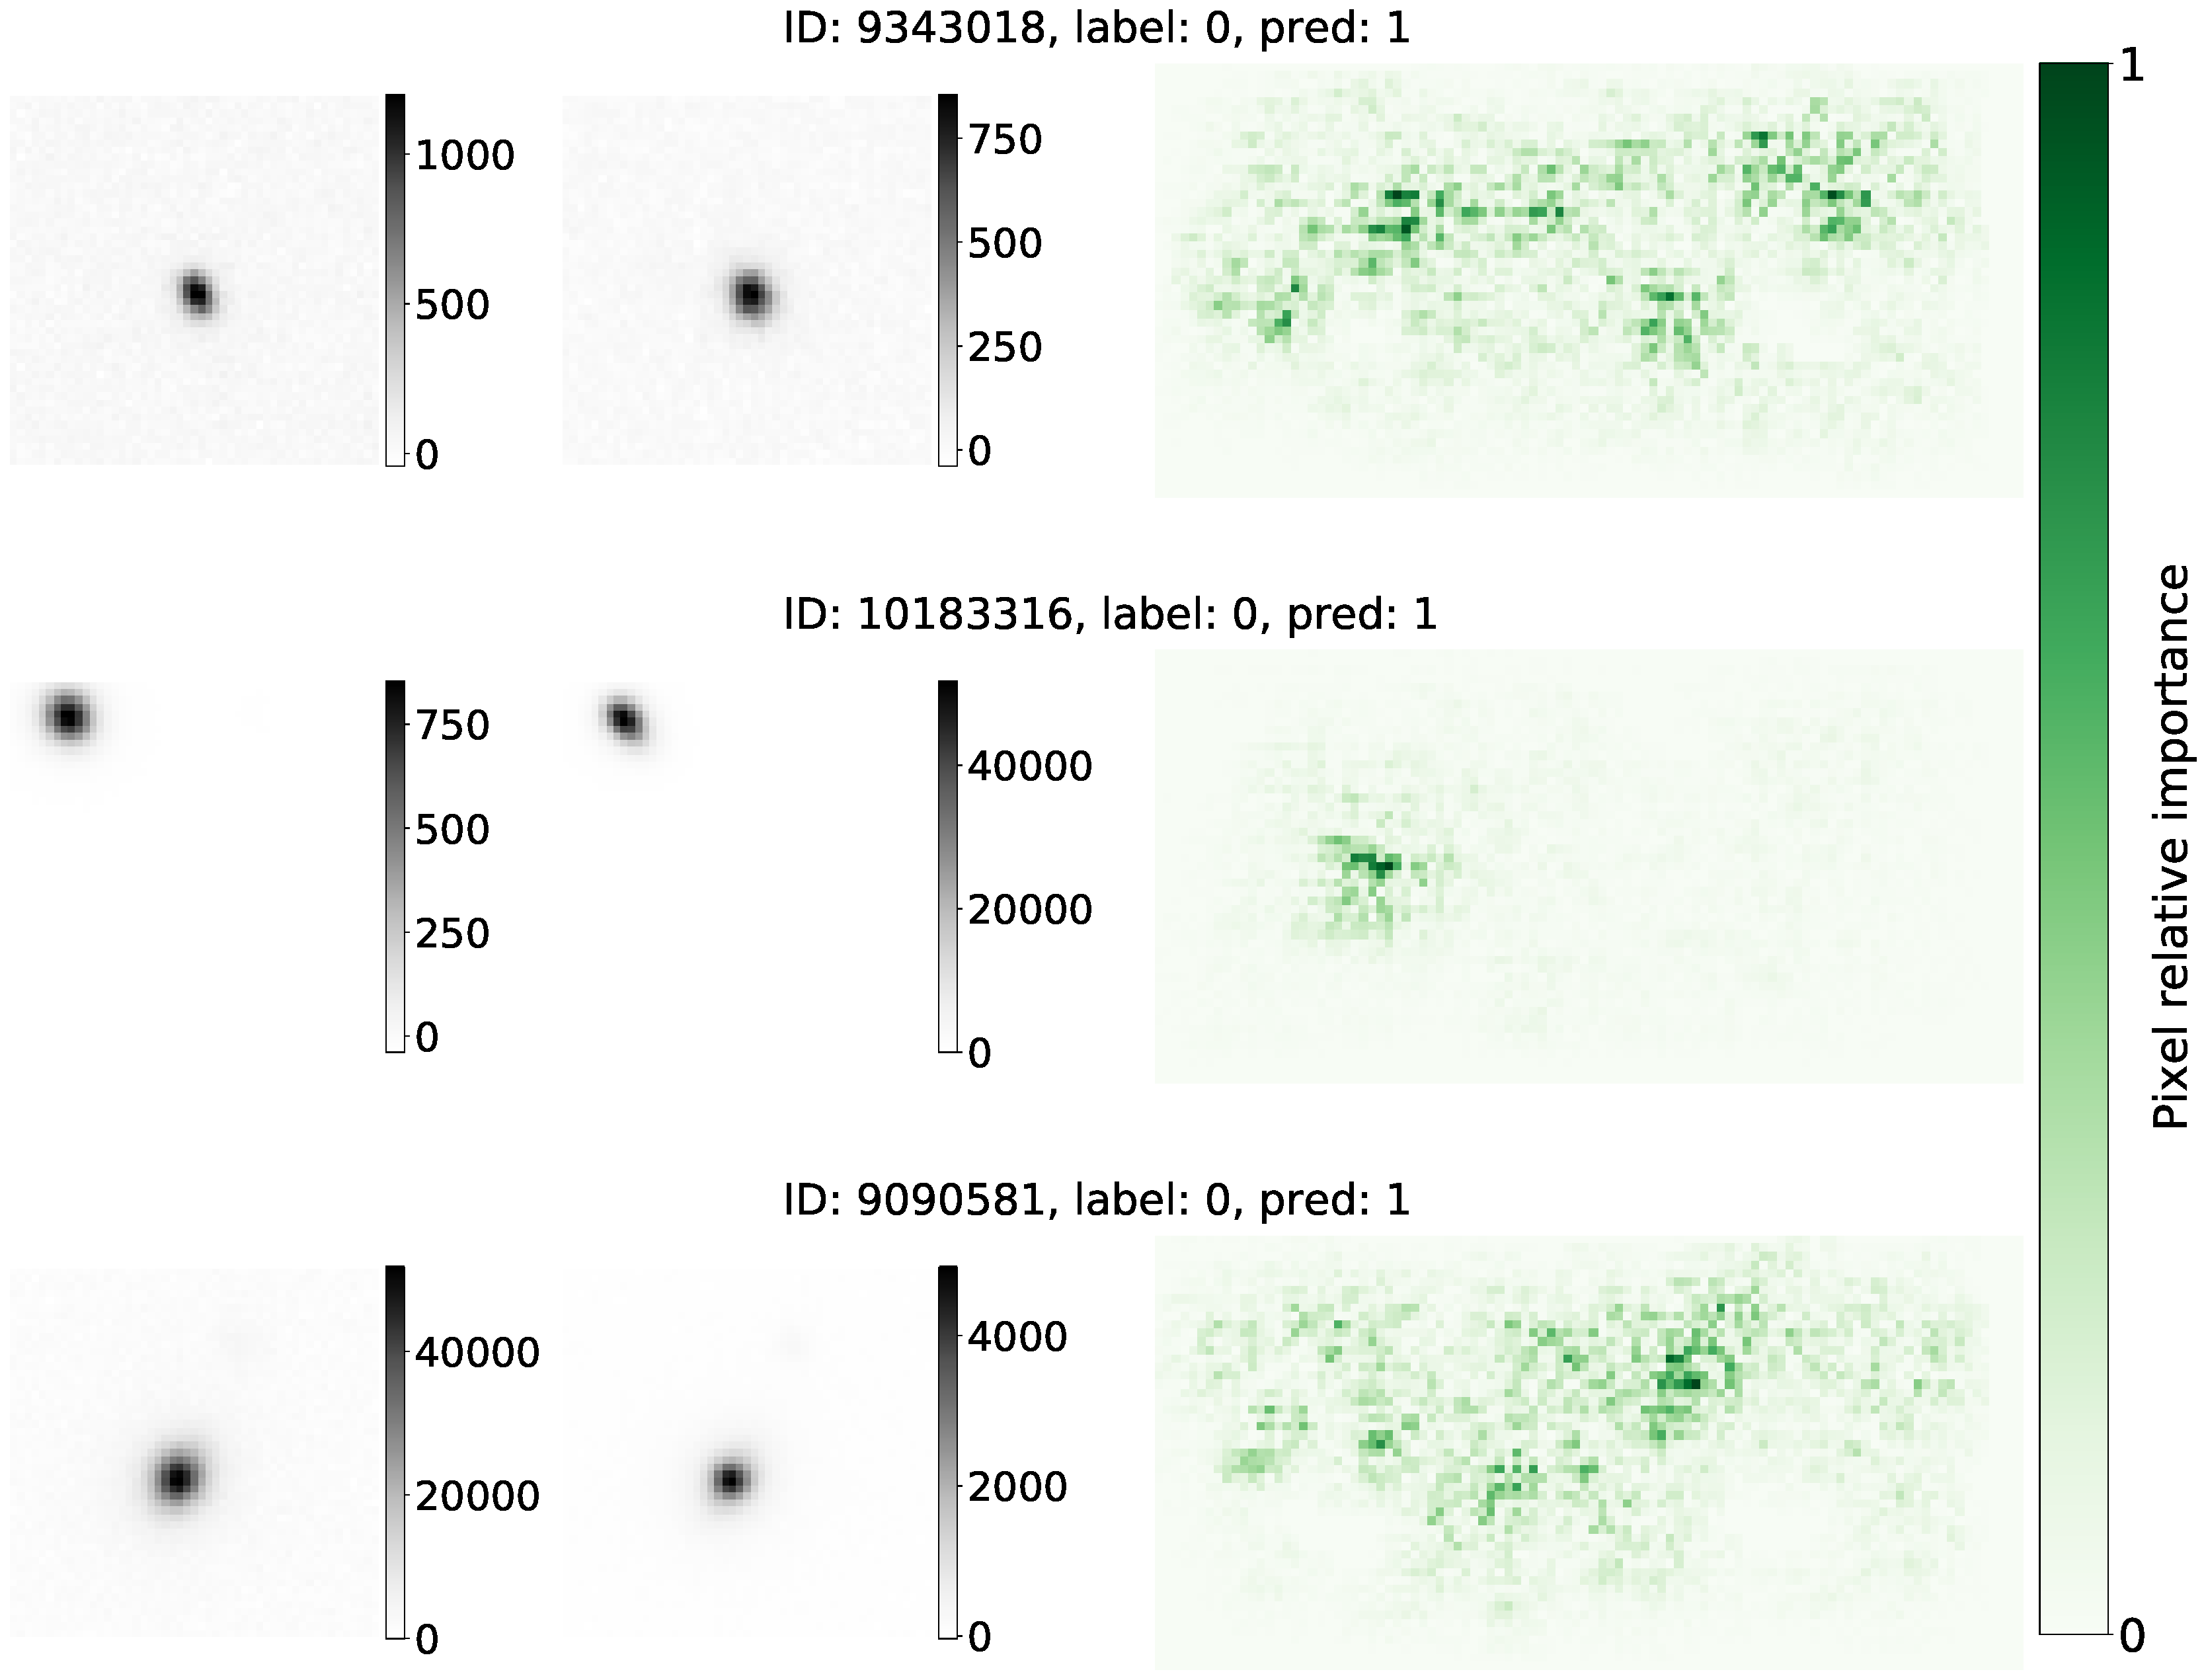
\includegraphics[width=0.76\linewidth]{
    figures/saliency_plot_other3nodiaFN-see981.pdf}
    \caption{
    Transients (\search-\temp) and their respective saliency map for the \nodia\ model False Negatives (astrophysical sources classified as ``bogus''). In all cases but row 5 it is not clear why the classification fails. In row 5, another source dominates the image scaling (and pre-processing) reducing the visibility of the transient (that is completely missed by human inspection). We remind the reader that the ``real'' transients in this dataset are implanted supernovae onto real DES images. Important pixels are found everywhere in the image, as the CNN learns how to compare the \diff\ and \temp\ taking a synoptic look at the properties of each image component.}
    \label{fig:fnndia}
\end{figure*}



\begin{figure*}
    \centering
    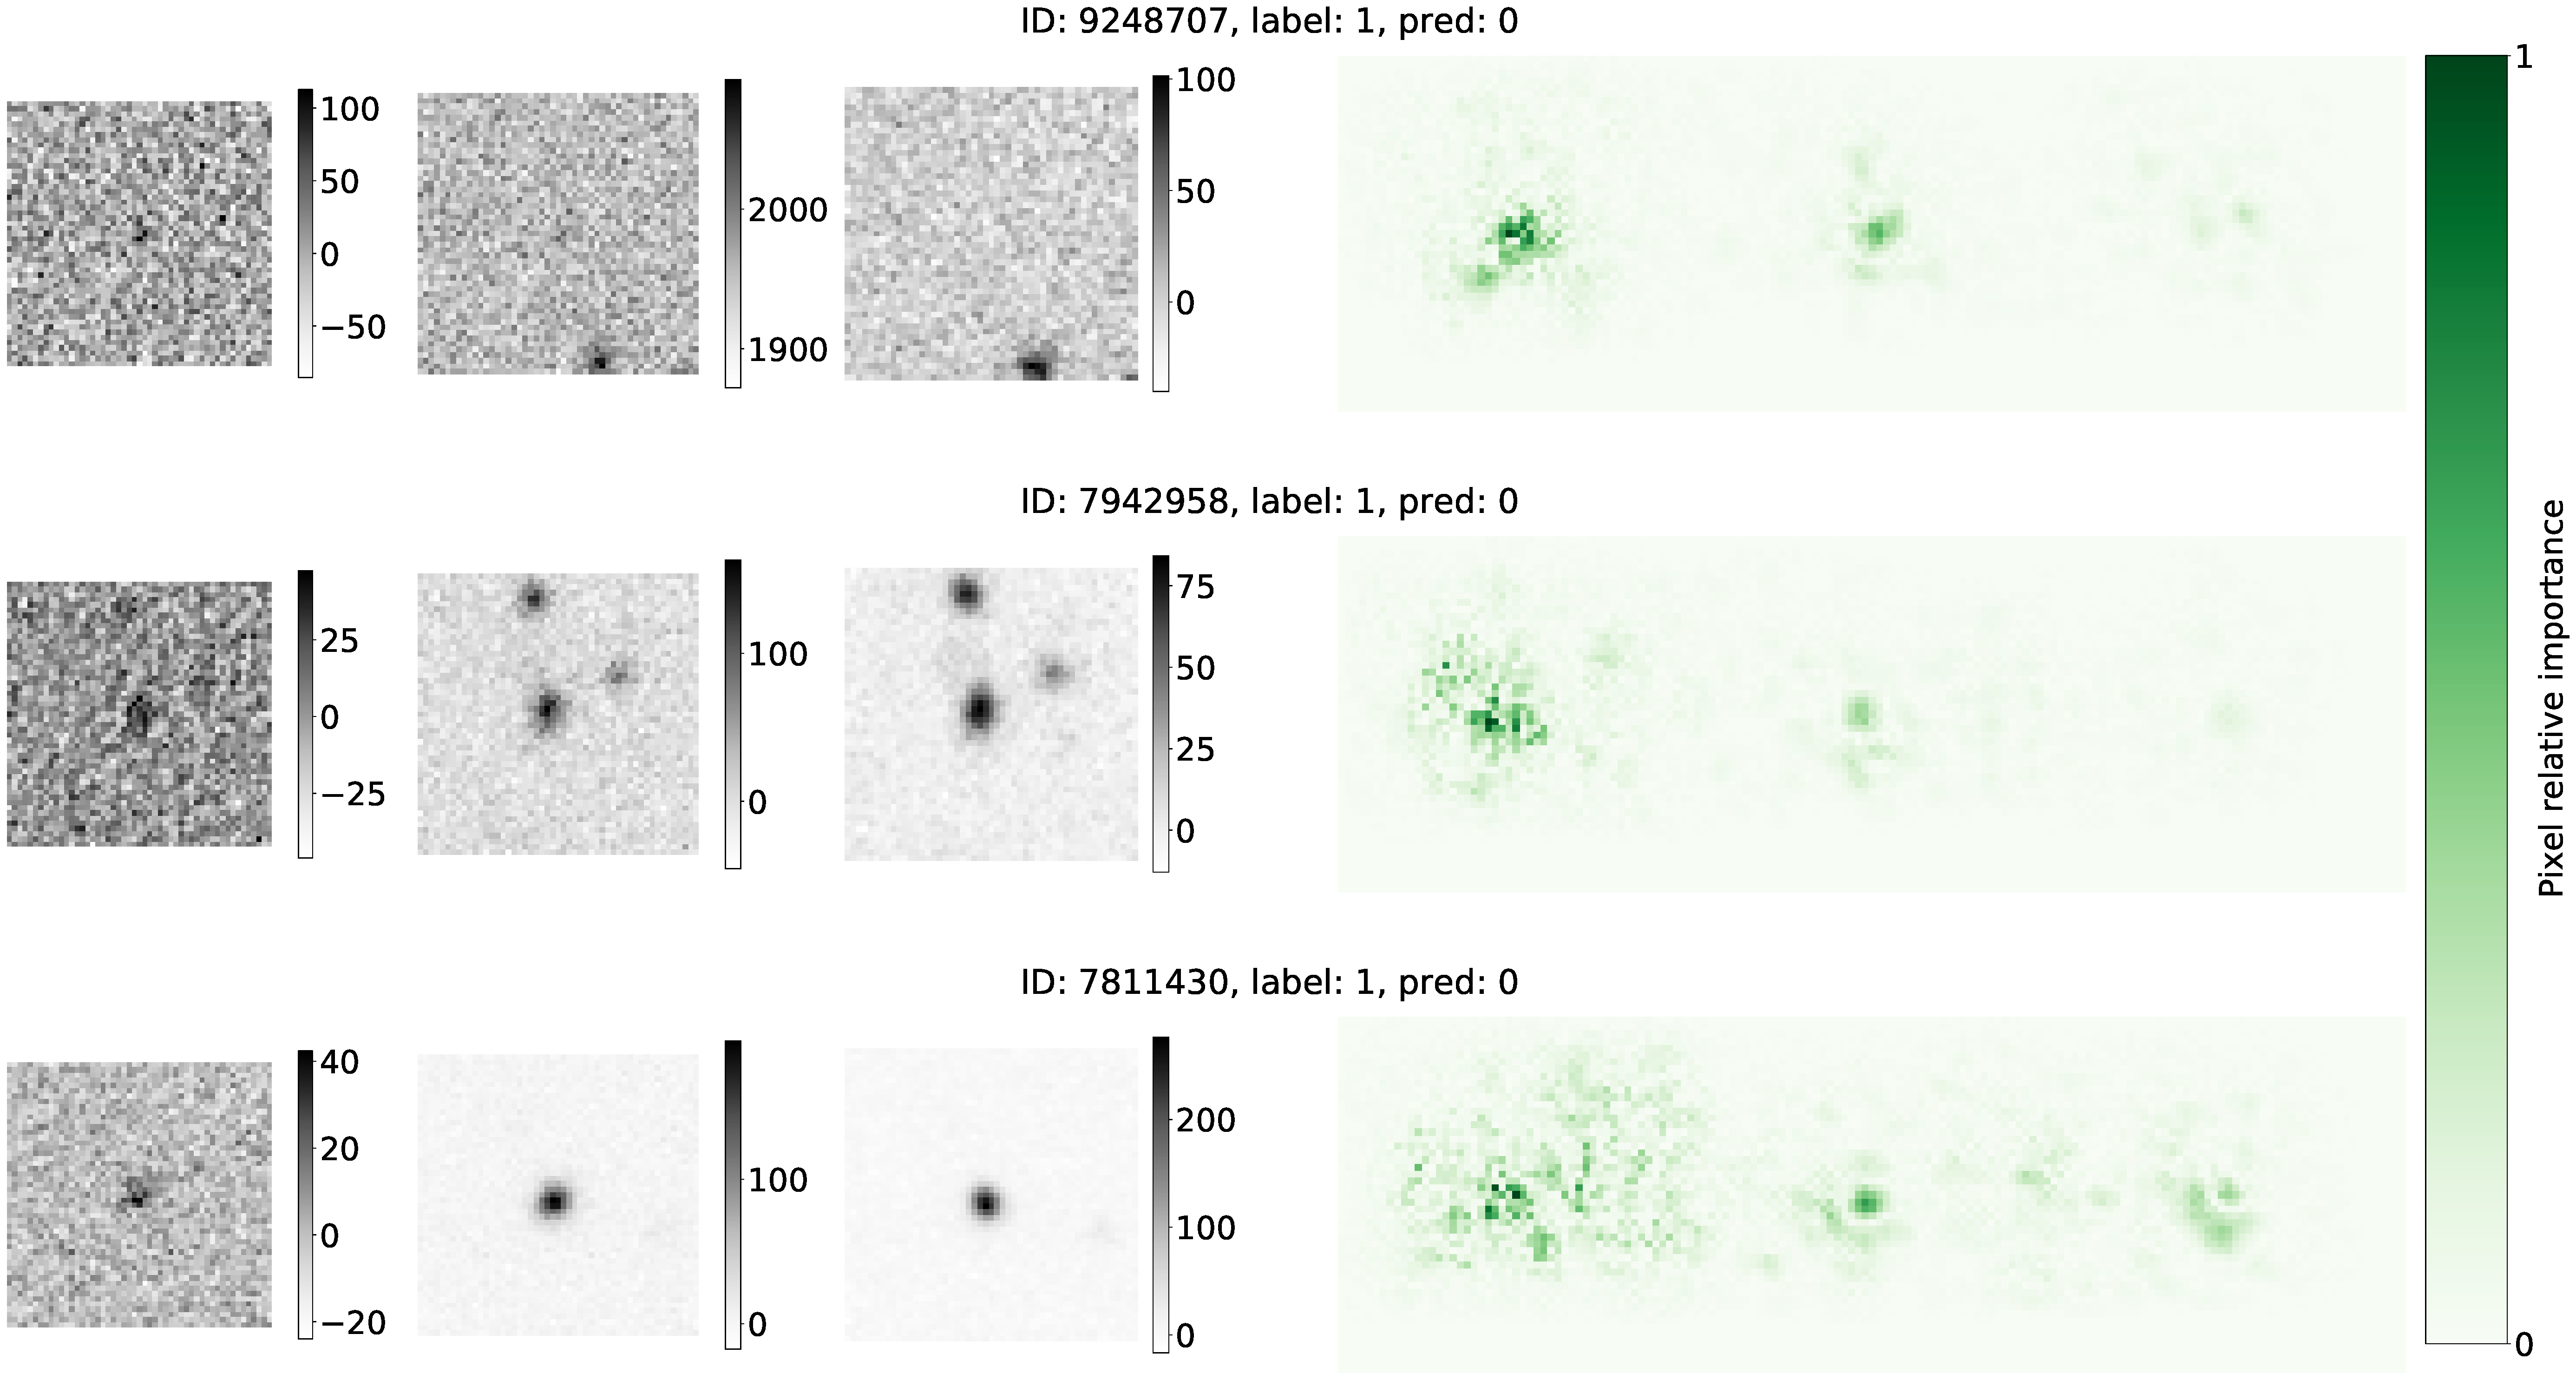
\includegraphics[width=0.8\linewidth]{
    figures/saliency_plot_other3FP-see21.pdf}
    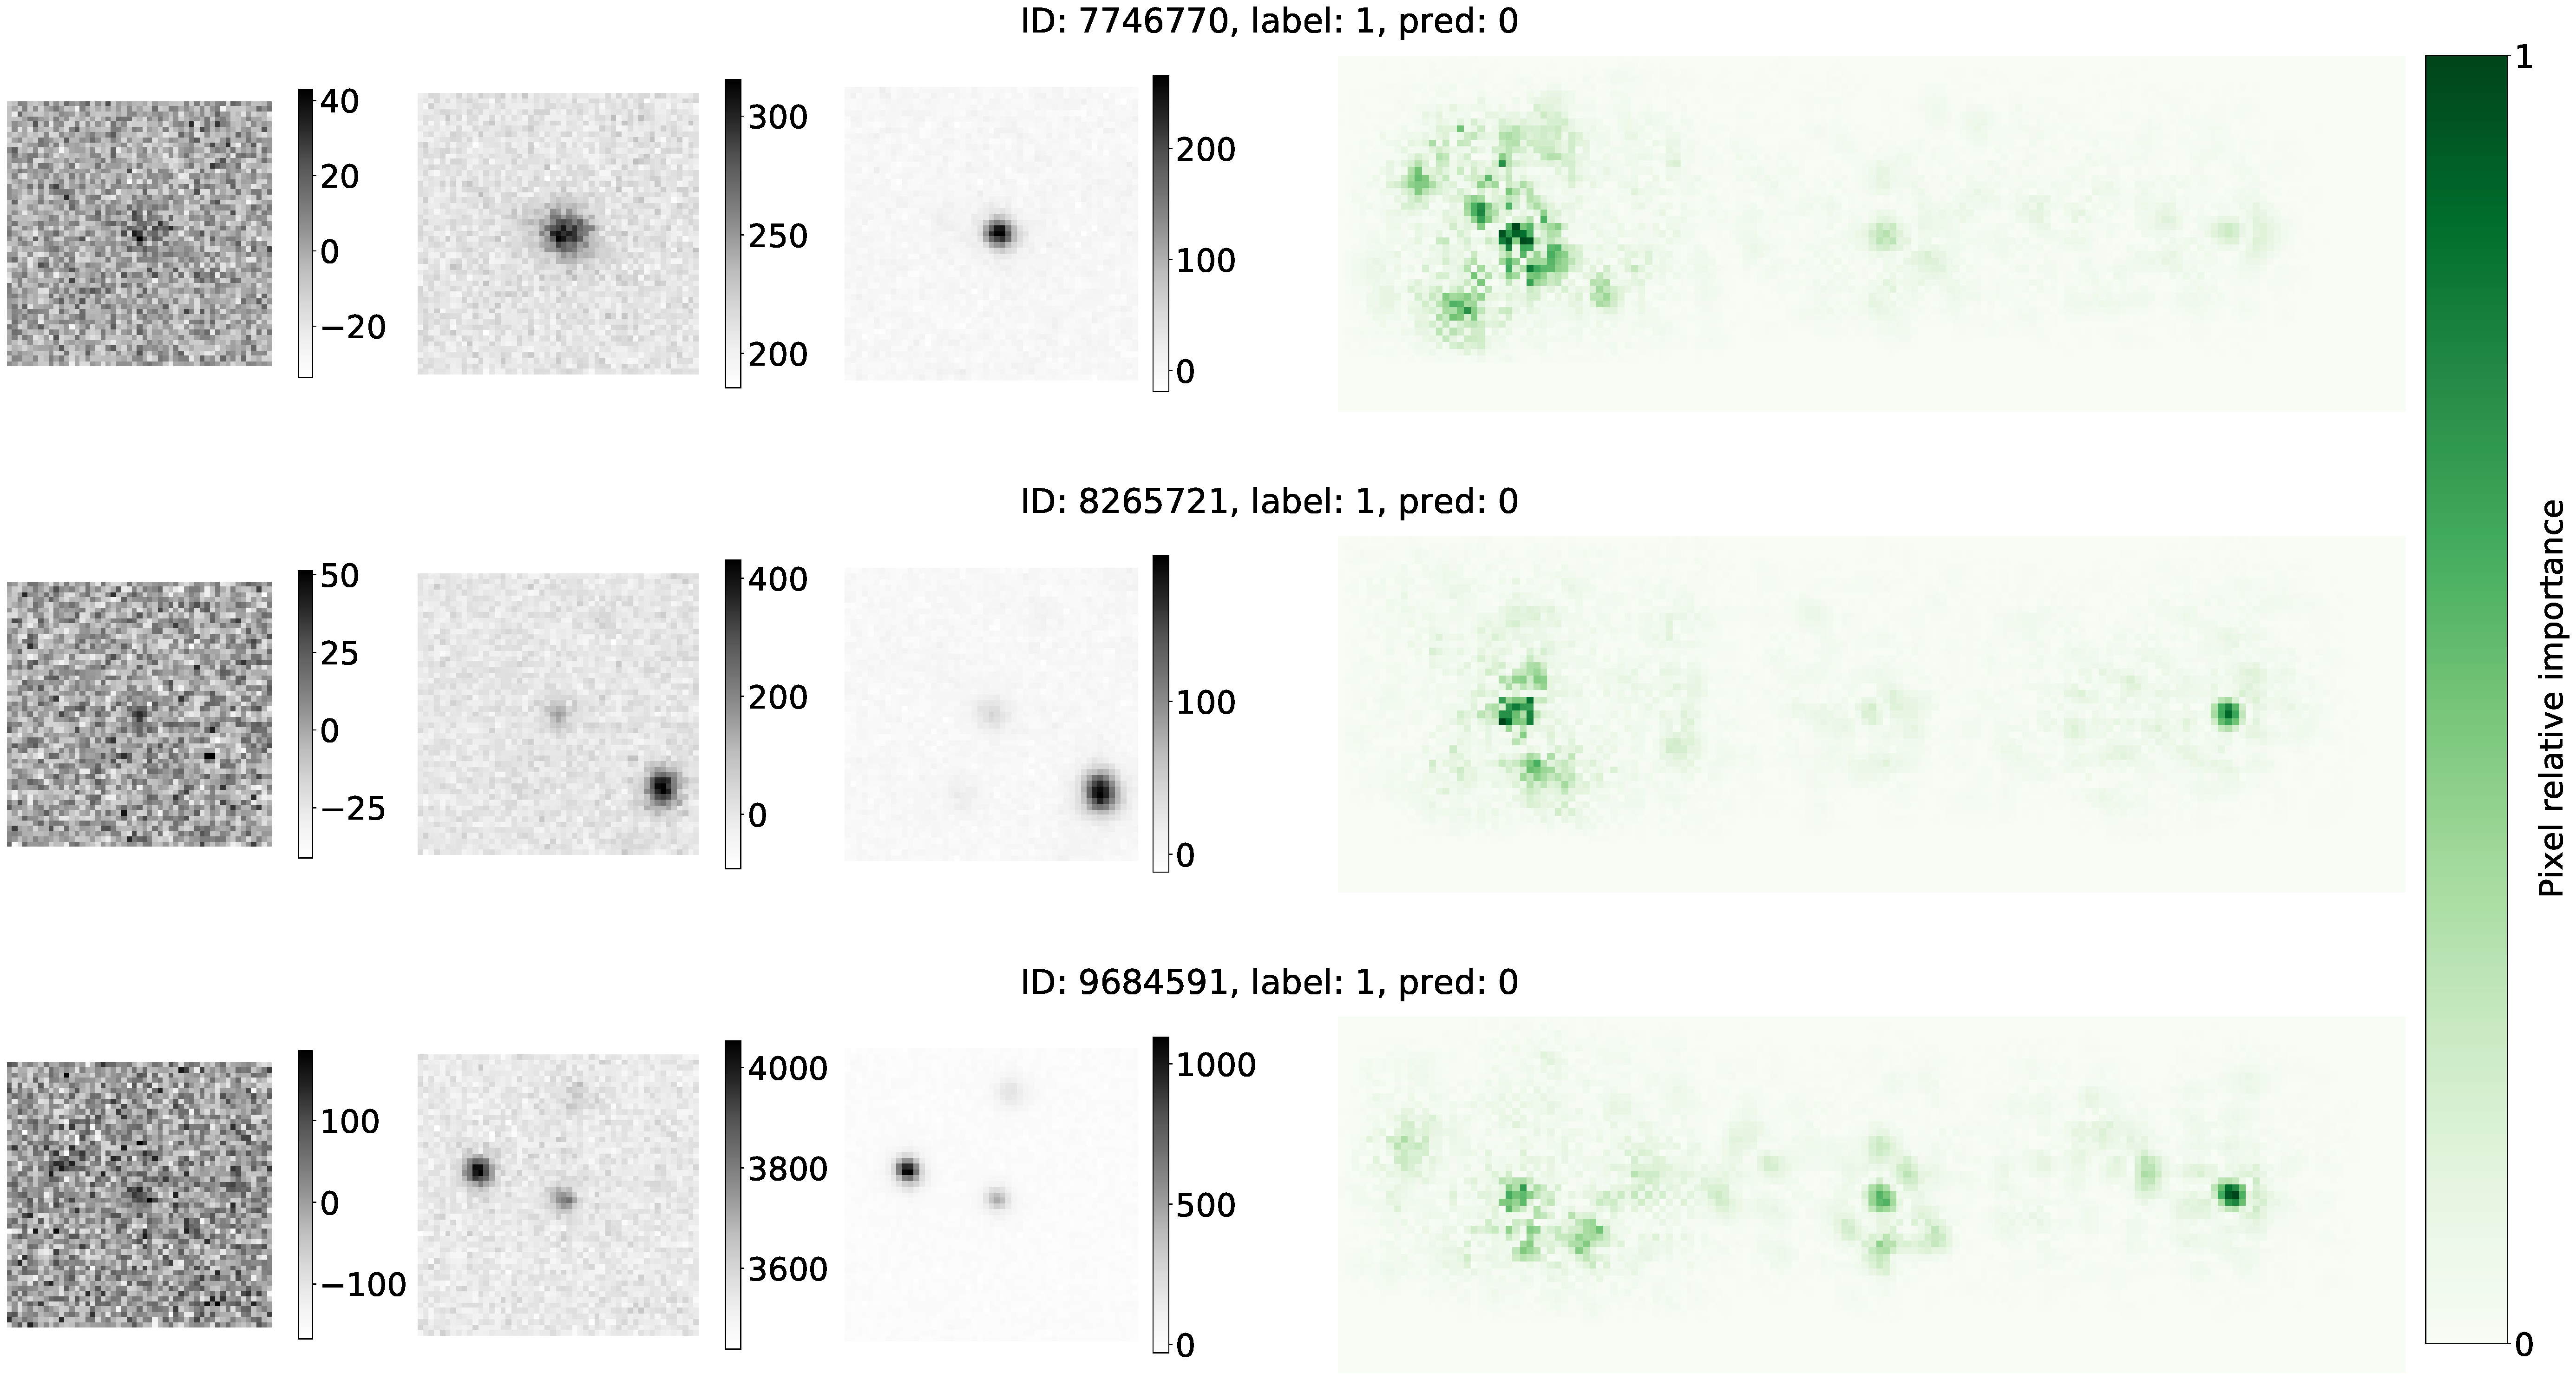
\includegraphics[width=0.8\linewidth]{
    figures/saliency_plot_other3FP-see369.pdf}
    \caption{Transients (\diff-\search-\temp) and their respective saliency map for \diabased\ model False Positives (``bogus'' predicted as ``real'').  We remind the reader again that the labels are inherited from  \citet{Goldstein_2015} and cannot be verified.  Some level of label inaccuracy is expected. Bogus transients were labeled by human scanners among astrophysical images with detection. However, in this collection, we cannot verify the nature of the transient and we argue that in the cases presented here there is no obvious evidence of its ``bogus'' nature. Important pixels are most commonly found in the \diff, but in \temp\ and \search\ we see again the CNN analyzes the central source and its surrounding, but avoiding the tail of the central source, in a way similar to traditional aperture photometry techniques.}
    \label{fig:saliency_dia3id_FP}
\end{figure*}
\begin{figure*}
    \centering
    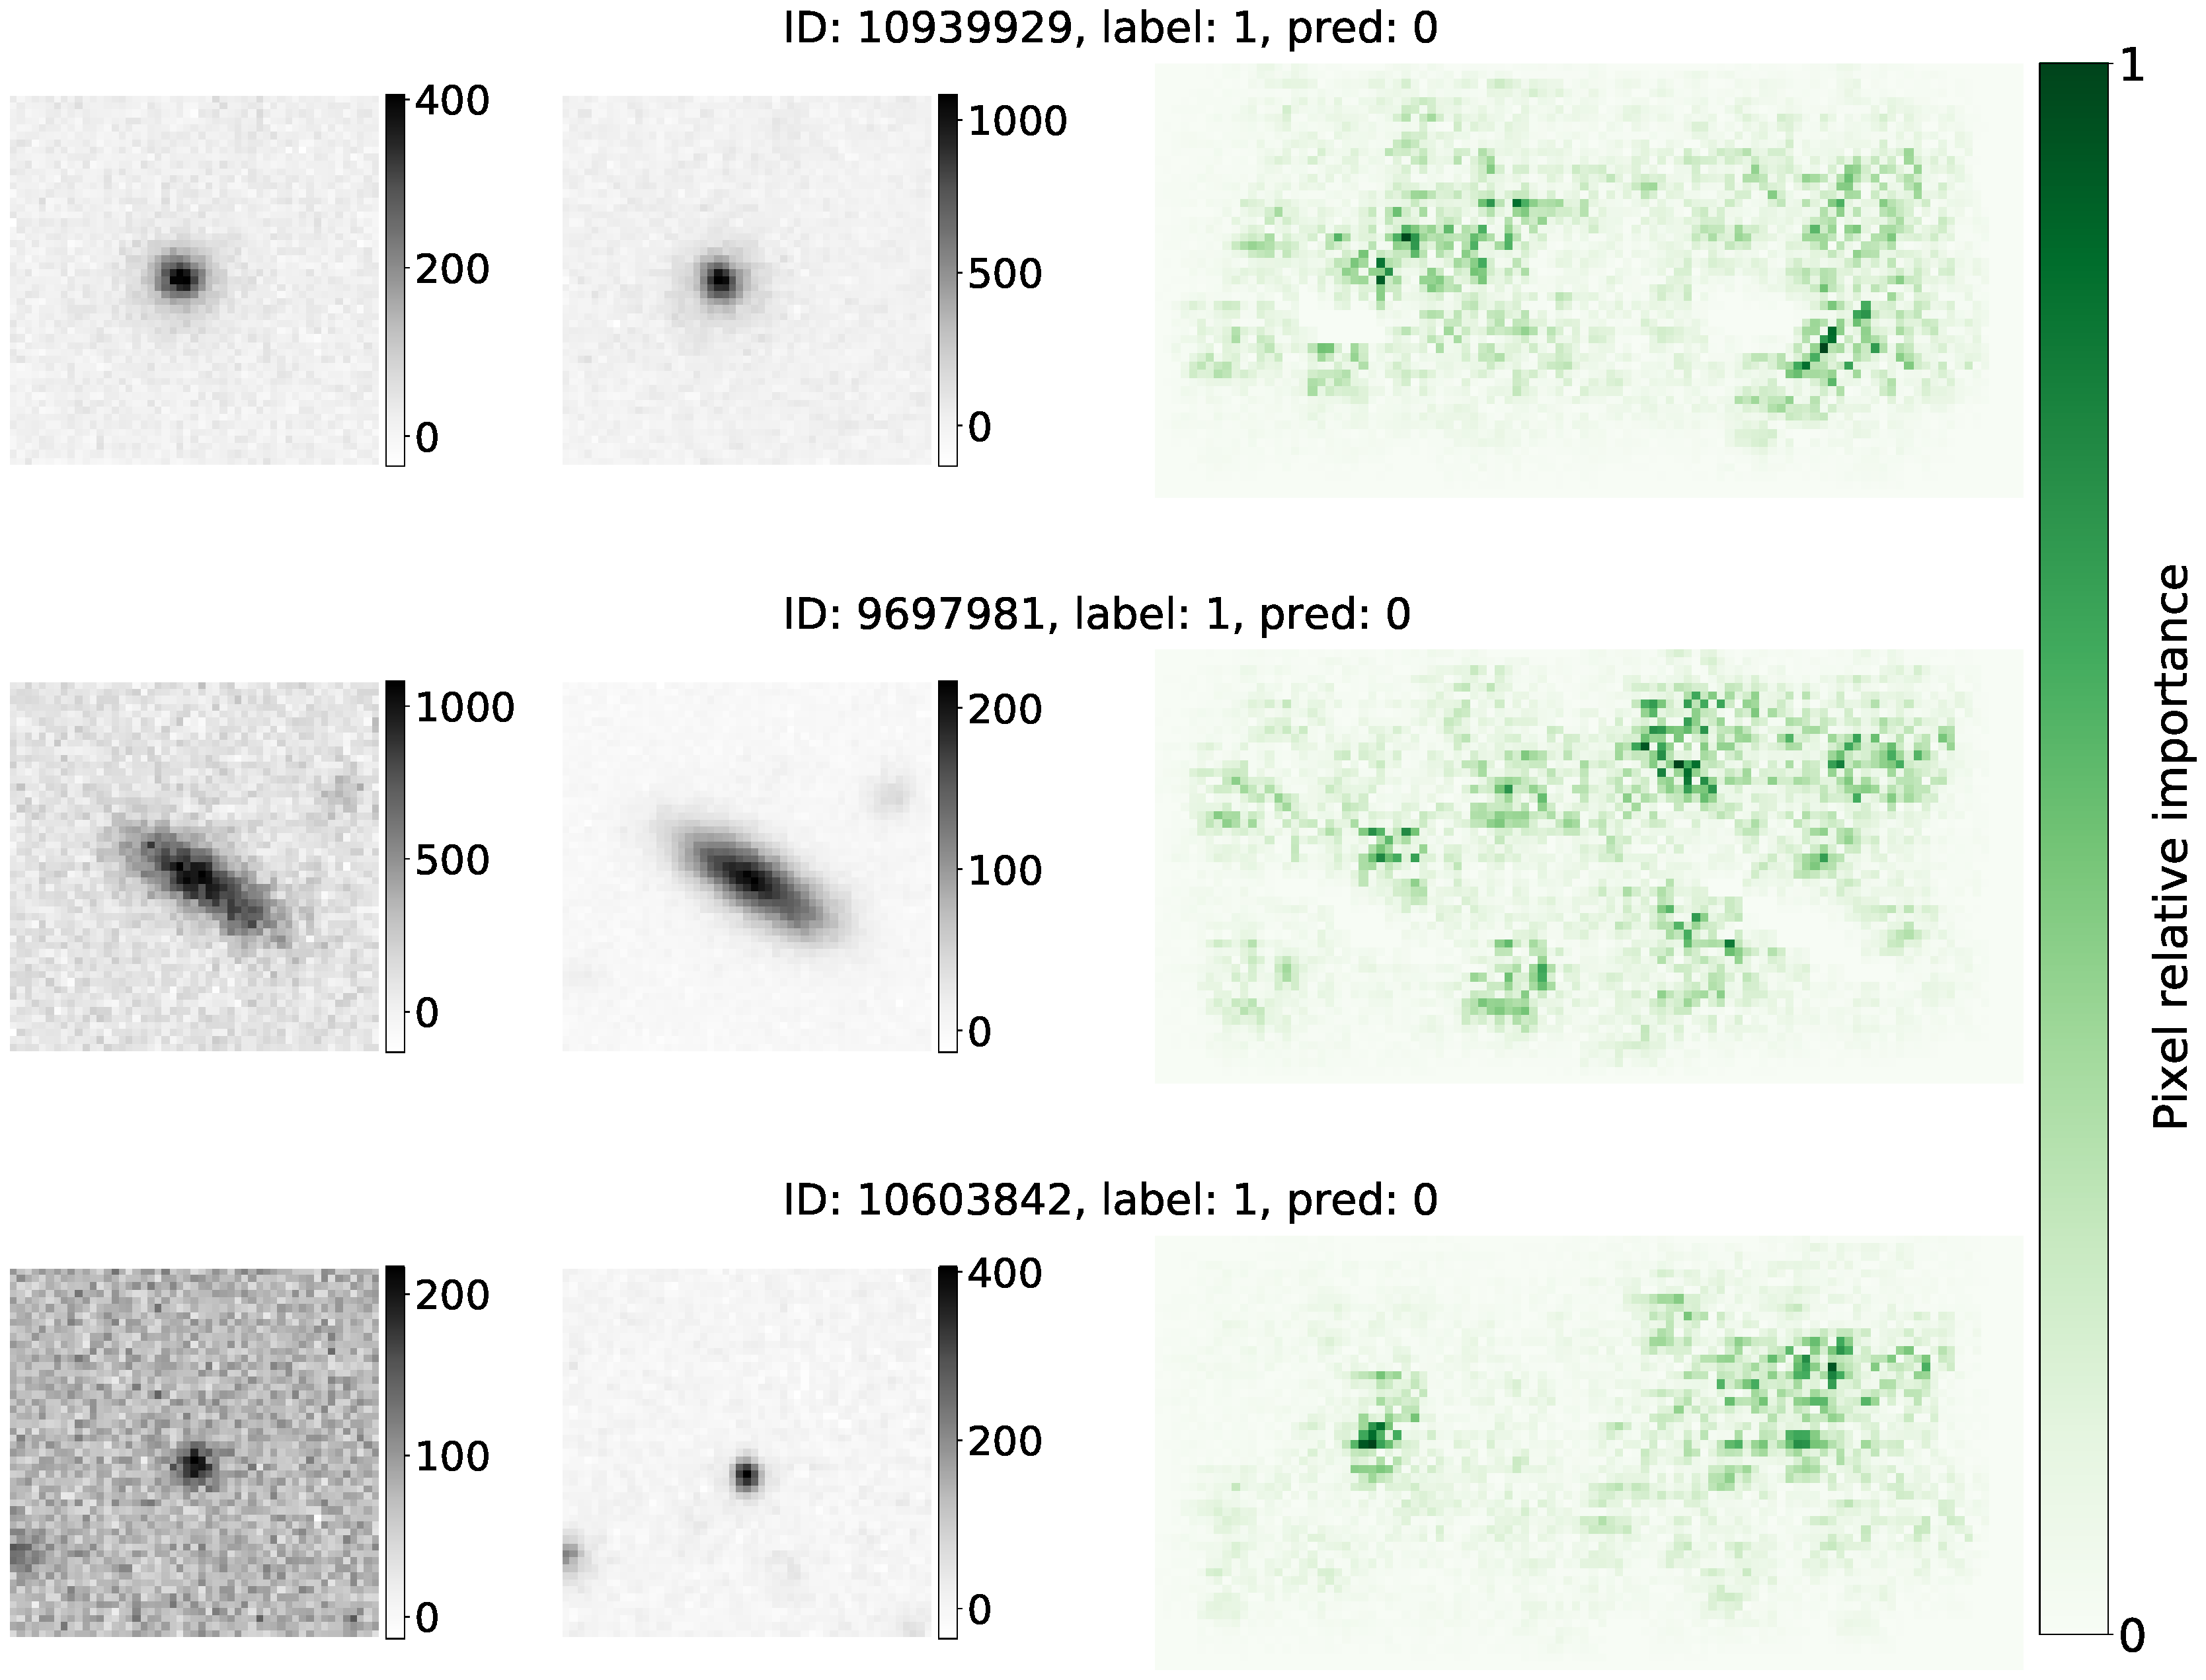
\includegraphics[width=0.76\linewidth]{
    figures/saliency_plot_other3nodiaFP-see18.pdf}
    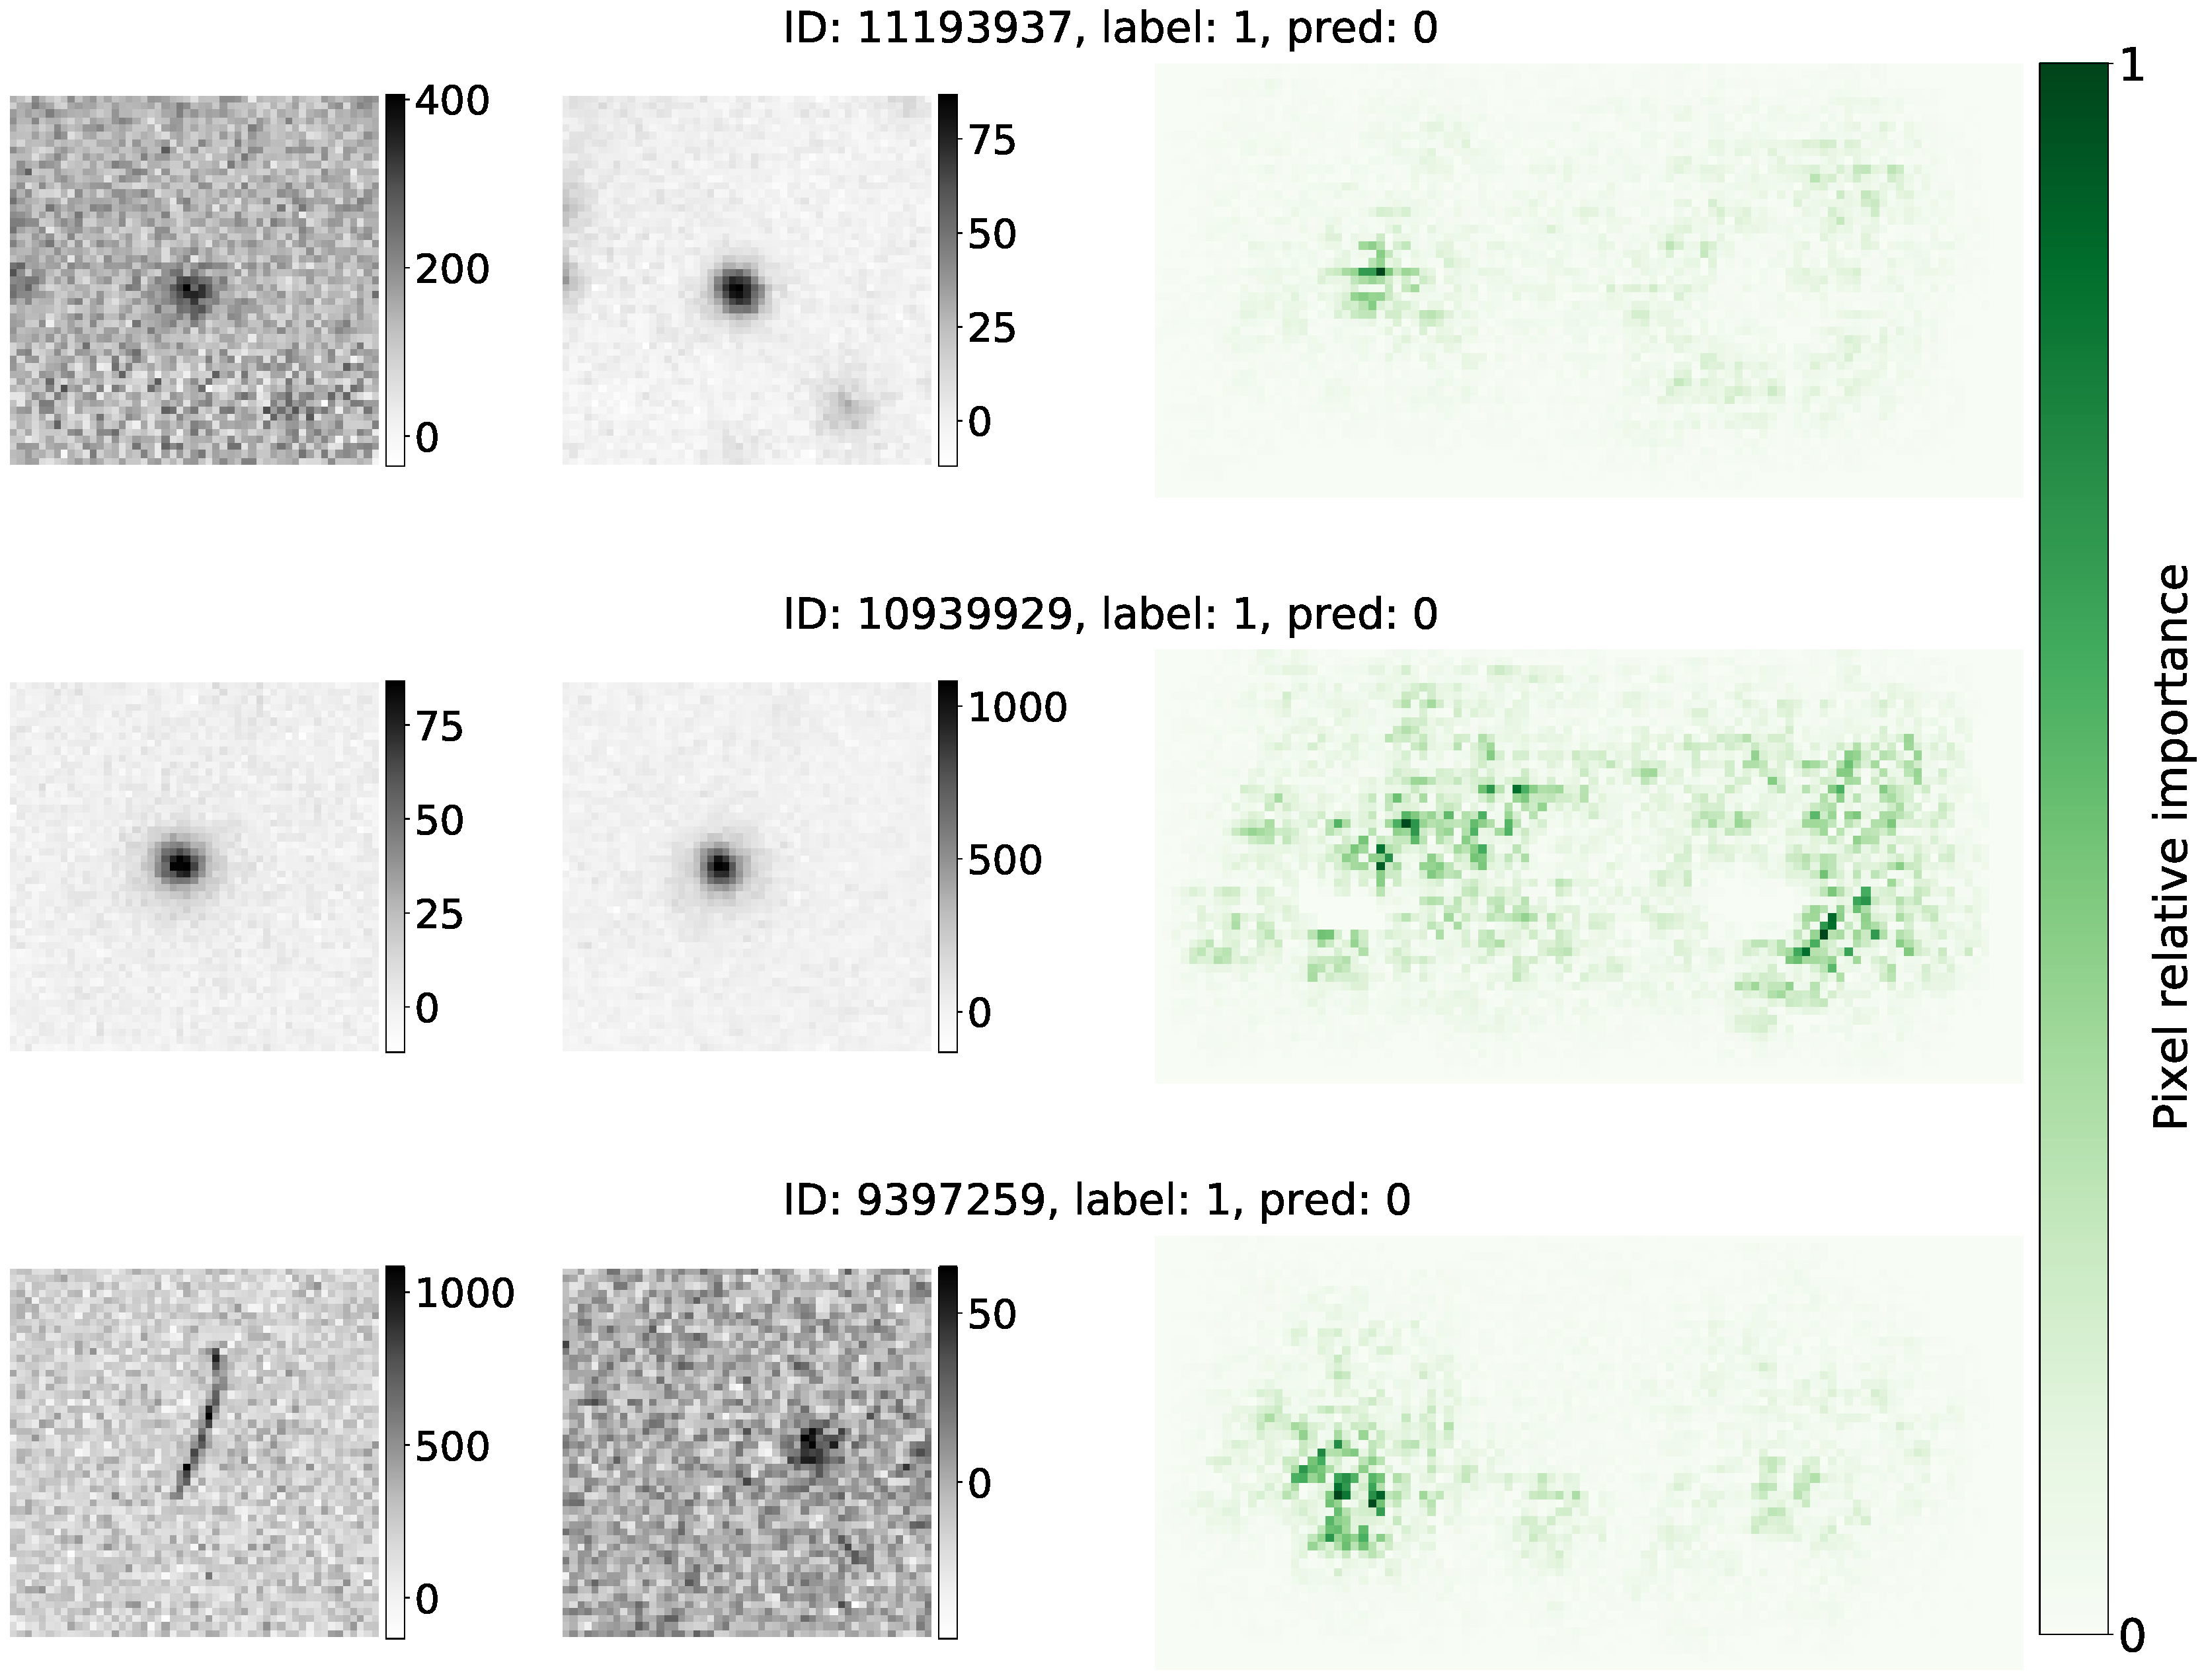
\includegraphics[width=0.76\linewidth]{
    figures/saliency_plot_other3nodiaFP-see854.pdf}
    \caption{Transients (\search-\temp) and their respective saliency map for the \nodia\ model False Positives (``bogus''  classified as ``real''). Important pixels are found everywhere in the image, as the CNN learns how to compare the \diff\ and \temp\ taking a synoptic look at the properties of each image component.}
    \label{fig:fpndia}
\end{figure*}